\clearpage
\appendix

%%%%%%%%%%%%%%%%%%%%%%%%%%
%APPENDIX
%%%%%%%%%%%%%%%%%%%%%%%%%%

\section{Appendix: Data sets}\label{appendix:data}
\setcounter{figure}{0}    
\setcounter{table}{0}    
\renewcommand*\thetable{\Alph{section}.\arabic{table}}
\renewcommand*\thefigure{\Alph{section}.\arabic{figure}}
\renewcommand{\theHfigure}{\Alph{section}.\arabic{table}}
\renewcommand{\theHtable}{\Alph{section}.\arabic{figure}}

We use 9 different data sets from 8 countries:

\begin{enumerate}
    \item Australia: Australia panel data are from the Household, Income and Labour Dynamics in Australia \citep{hilda_household_2022}.  HILDA is a longitudinal survey that has been following members of a nationally representative sample of Australian households on an annual basis since 2001 \citep{watson_wooden_2012}.  In 2001, the survey contained data on nearly 14,000 individuals in nearly 7,700 households.  As of 2018, the HILDA Survey included data from approximately 17,500 individuals in around 9,500 households across Australia.  The HILDA Survey includes information about employment and earnings for sample participants that are 15 years or older.  

    \item Germany: German panel data are from the Socio-Economic Panel \citep{soep_2020}.  SOEP is a longitudinal study of private households in Germany.  The survey is conducted annually.  Sample A, often called the `West German Sample', began in 1984 and included West Germany, both Germans and foreigners.  Sample B, `Foreigners in the Federal Republic of Germany', was also created in 1984 in order to over sample foreigners that were under represented in Sample A.  Sample C was begun in 1990 to include German residents of the German Democratic Republic (GDR).  Since then, numerous refresher samples were added in order to supplement panel attrition \citep{soep_jan_2019}.  In 2000, the SOEP included data from around approximately 22.000 individuals in 12,000 households. By 2018, the SOEP contained information from about 32,000 individuals in about 19,000 households across Germany.

    \item Italy: Since the 1960s, the Bank of Italy has conducted the Survey on Household Income and Wealth  \citep{shiw_historical_2019} biannually. Its primary objective is to amass comprehensive data regarding the individual and households family composition and employment status.   Since 1989, the sample included households previously interviewed going back to 1977.  However, the survey only includes data on contract type since 2000.  In 2000, the survey included data on approximately 14,000 individuals in 8,000 households.  By 2016, the survey includes data on nearly 70,000 individuals in nearly 40,000 households.  As we noted in the main document, we do not include panel data after 2016.  In 2022, The Bank of Italy released the 2022 survey wave for SHIW, which contains data up to 2020, but skips the 2020 biannual survey wave, which would have contained data up to 2018.  As a result, if we were to use the 2022 wave, there would be a four-year gap between 2020 and 2016, not a two-year gap between 2020 and 2018 or 2018 and 2016 as should be the case if the 2020 panel wave was released.

    \item Japan: Japanese panel data are harmonized from the Keio Household Panel Survey and the Japan Household Panel Survey \citep{jhpskhps_keio_2019}.  Both are annual surveys.  The KHPS has been implemented annually since 2004 on 4,000 households and 7,000 individuals nationwide.  In 2009, the JHPS began as a new survey targeting 4,000 male and female individuals in parallel with the KHPS.  The two data sets are harmonized prior to release by the agency responsible for making the data available to researchers.  As of 2018, the survey includes data on nearly 10,000 individuals.  

    \item Korea: Korean panel data are from the Korea Labor and Income Panel Study \citep{klips_korean_2020}.  It is an annual survey of urban households members who are at least 15 years of age or older that began in 1998.  In 1999, the first year it included data on approximately 13,000 individuals in 5,000 households.  By 2018, the survey includes data on nearly 25,000 individuals.

    \item Netherlands: We use two panel data sets for the Netherlands.  
    \begin{enumerate}
        \item Arbeidsaanbodpanel or Labour Supply Panel \citep{lsp_arbeidsaanbodpanel_2016} - We use the LSP as our main source of panel data.  Begun in 1985, it is a biannual long-term survey of the Dutch working population (aged 16 - 66) and their employment situation.  Unfortunately, the LSP ended in 2014.
        \item Longitudinal Internet Studies for the Social Sciences \citep{liss_longitudinal_2020} - We use the LISS as a sensitivity for the LSP.  The LISS is not a replacement for the LSP.  Begun in 2007, it is an annual survey of 5,000 households, comprising approximately 7.500 individuals, 16 years of age or older.  Unique among all other panel data, panel participants complete online questionnaires every month.  As a result, non-internet users are absent.  Without denying the advantages and value of the LISS, the survey does suffer from high levels of panel attrition, as shown in table \ref{table_sample_filter_steps_country_NE}.
    \end{enumerate}

    \item Switzerland: Swiss panel data are from the Swiss Household Panel \citep{shp_swiss_2020}.  The SHP is conducted by the Swiss Foundation for Research in Social Sciences (FORS).  Available since 1999, it is an annual survey that interviews all household members over the age of 14 from a random sample of private households in Switzerland, stratified across the seven major statistical regions of Switzerland.  The SHP combines three samples: the SHP I (5,074 households and 7,799 individuals interviewed first in 1999), the SHP II (2,538 households and 3,654 individuals interviewed first in 2004) and the SHP III (3,989 households and 6,090 individuals interviewed first in 2013).  In total, there are nearly 16,000 individuals in nearly 10,000 households.  

    \item United Kingdom: Panel data from the United Kingdom are harmonized from the British Household Panel Study (BHPS) and the United Kingdom Household Longitudinal Study \citep{bhpsukhls_university_2022}.  Both are annual surveys.  Begun in 1991, the BHPS followed the same representative sample of individuals.  In 2008, as part of wave 18, BHPS participants were asked if they would consider joining the new, larger, more wide-ranging survey called Understanding Society or UKHLS.  Therefore, the UKHLS is considered a supplement and extension of the original BHPS.  BHPS and UKHLS data are harmonized, allowing researchers to analyze data since 1991.

\end{enumerate}

With the exception of panel data from the Netherlands and Italy, most of our data are available in the CNEF.  As noted by Tillmann et al. \citeyearpar[pg. vii]{tillmann2018social}, ``The fact that the panels in CNEF are comparable is not a lucky accident, but rather an important feature of the worldwide social and behavioral sciences research infrastructure. A concerted effort ensures that these panel studies are comparable in terms of the basic setups and the questionnaires.''  

%%%%%%%%%%%%%%%%%%%%%%%%%%%%%%%%%%%%%%%%%%
%%%%%%%%%%%%%%%%%%%%%%%%%%%%%%%%%%%%%%%%%%
%%%%%%%%%%%%%%%%%%%%%%%%%%%%%%%%%%%%%%%%%%
%%%%%%%%%%%%%%%%%%%%%%%%%%%%%%%%%%%%%%%%%%

\clearpage
\setcounter{table}{0}
\setcounter{figure}{0}
\renewcommand*\thetable{\Alph{section}.\arabic{table}}
\renewcommand*\thefigure{\Alph{section}.\arabic{figure}}
\renewcommand{\theHfigure}{\Alph{section}.\arabic{table}}
\renewcommand{\theHtable}{\Alph{section}.\arabic{figure}}

\section{Appendix: Recoding variables}\label{appendix:variables}

One cannot dismiss the methodological challenges associated with comparing data from national panel surveys given large differences in sampling and survey design. Input harmonized is the process of standardizing or normalizing data inputs before they are collected and entered into a system to ensure that data collected from different sources follow a standardized format and coding scheme (i.e. EU-SILC).  By contrast, output harmonized is the process of recoding the data after it has been collected in order to align data to a common set of variables, codes, and classification.  While CNEF/CPF refer to their data as `harmonized,' they may be better characterized as output harmonized and accurately understood as recoding, as we do here.  

In order to compare across variables in different data sets, we recoded five variables: employment status, employment contract, hours, wages and salary from a person's main job, education.  With the exception of top codes and missing cases, four variables require no recoding: age, gender, person ID, year.  

We also include a variable for country-level unemployment rate, which comes from World Bank data, not OECD because OECD does not include Switzerland before 2010, after 2010, both data sources are the same. 

The dependent variable is log of hourly wages.  To create a variable for hourly wage, hours and wages are recoded into monthly values to compare across data sets.  Wages are either monthly or annually, but hours are often weekly, with the exception of Germany where hours are annual.  Hourly wages are created by dividing monthly wages by monthly hours worked.    Once we create a variable for hourly wages, wages are inflation adjusted to the year 2010 using the country-specific, CPI index from the World Bank.  Wages are represented in the national currency and are not adjusted using any equivalence scale.  

Employment status is recoded into a categorical variable with two levels indicating, employed or unemployed and looking for work.  This is shown in figure \ref{graph_descriptives_emp_status}.  Unemployment is variously defined by country.  If not stated, then we assume that `unemployed' is defined as unemployed, but looking for work.  We do not use additional survey items on whether a respondent is looking for work while being unemployed.  

Employed is further specified as an individual with an observable contract type with observable monthly hours between 40 and 320 (i.e. no less than 10 hours per week and no more than 80 hours per week.


Education.  We do not control for education as it is usually time-invarying for adult participants in the labour force.  However, we do split the analysis by education group as a sensitivity test (see Appendix \ref{appendix:sensitivity_heterogeneity}.  Most countries use ISCED, but some countries do not.  For example, Germany uses CASMIN, Australia codes educational attainment in accordance with the Australia Bureau of Statistics (ABS) approach, and the Netherlands and Japan use their own definition.  Education is recoded into a categorical variable with three levels indicating, less than secondary education, secondary education, and more than secondary education.  This is shown in figure \ref{graph_descriptives_education}.

The remaining variable is employment contract.  We measure temporary employment following OECD/Eurostat definitions to indicate if a contract is `permanent' or  `not permanent,' i.e. temporary in some way.  This is shown in figure \ref{graph_descriptives_contyp}.  

The single country exception is Australia, where we define `not permanent' as a fixed term contract (FTC).  This definition excludes casual work, a distinct type of employment relationship that is less comparable to temporary work in other countries because it offers a wage premium in exchange for the loss of other benefits \citep{mooi-reci_casual_2017}.  However, results over time after the first period are qualitatively similar if we include casual employment (as shown in the Appendix \ref{appendix:sensitivity_variable}, figure \ref{graph_sensitivity_AU}).  

If we exclude missing or unknown levels, then three countries, Switzerland (variable: pw36), Germany (variable: plb0037), and Korea (variable: p\_\_0501) use a single variable to ask whether the job duration is limited in some way, yes or no.  In Switzerland, a separate variable is used to specify the limited nature of the contract (variable pw37: apprenticeship, trial period, etc.).  For details on Switzerland, see figure \ref{graph_ch_compare_sample_age} in Appendix \ref{appendix:sensitivity_sample}.

Another five countries split temporary into two categories.  In Australia (variable: gjbmcnt), temporary employment is defined as either a `fixed term contract' or `casual basis'; in Italy (variable: contratt), temporary employment is defined as `fixed term' or `temporary'; in the Netherlands (variable: eb002), temporary employment is defined as either `temporary to permanent' or  `temporary'.  In Japan, employment status (v219) is split into seven categories, of which three are temporary: `contract employee', `subcontracted worker', and `specialized contract employee'.  

In the United Kingdom, before 1999, (variable: jbterm), temporary employment is defined as `seasonal/tmp' or  `contract/fixed time', after 1999 (variable: jbterm1), there is only permanent and not permanent.  Instead, like in Switzerland, a separate variable is used to specify the limited nature of the contract (variable jbterm2:).  Using jbterm2, we can distinguish work that is `Done under contract for a fixed period or a fixed task' from other types of temporary work, `seasonal', `agency', `casual', etc.  However, results are qualitatively similar if we include isolate temporary work that is done under a fixed term contract, form other types of temporary work (as shown in the Appendix \ref{appendix:sensitivity_variable}, figure \ref{graph_sensitivity_UK}).  

Unlike Australia or the United Kingdom, we do not perform a similar sensitivity check for Switzerland because all temporary work is a fixed-term contract that is limited in duration by time.

We do not suggest that temporary or permanent contracts are the same between countries nor do we suggest that all temporary contracts are the same within countries.  For this reason, wages of temporary workers are not directly compared across countries, but within countries and within persons in comparison to permanent work and unemployment.  Instead, the key point is that there is a bigger difference between permanent and temporary contracts than within temporary contracts.  

\begin{sidewaysfigure}[h!]
    \caption{Recode employment status by country}
    \resizebox{\textwidth}{!}{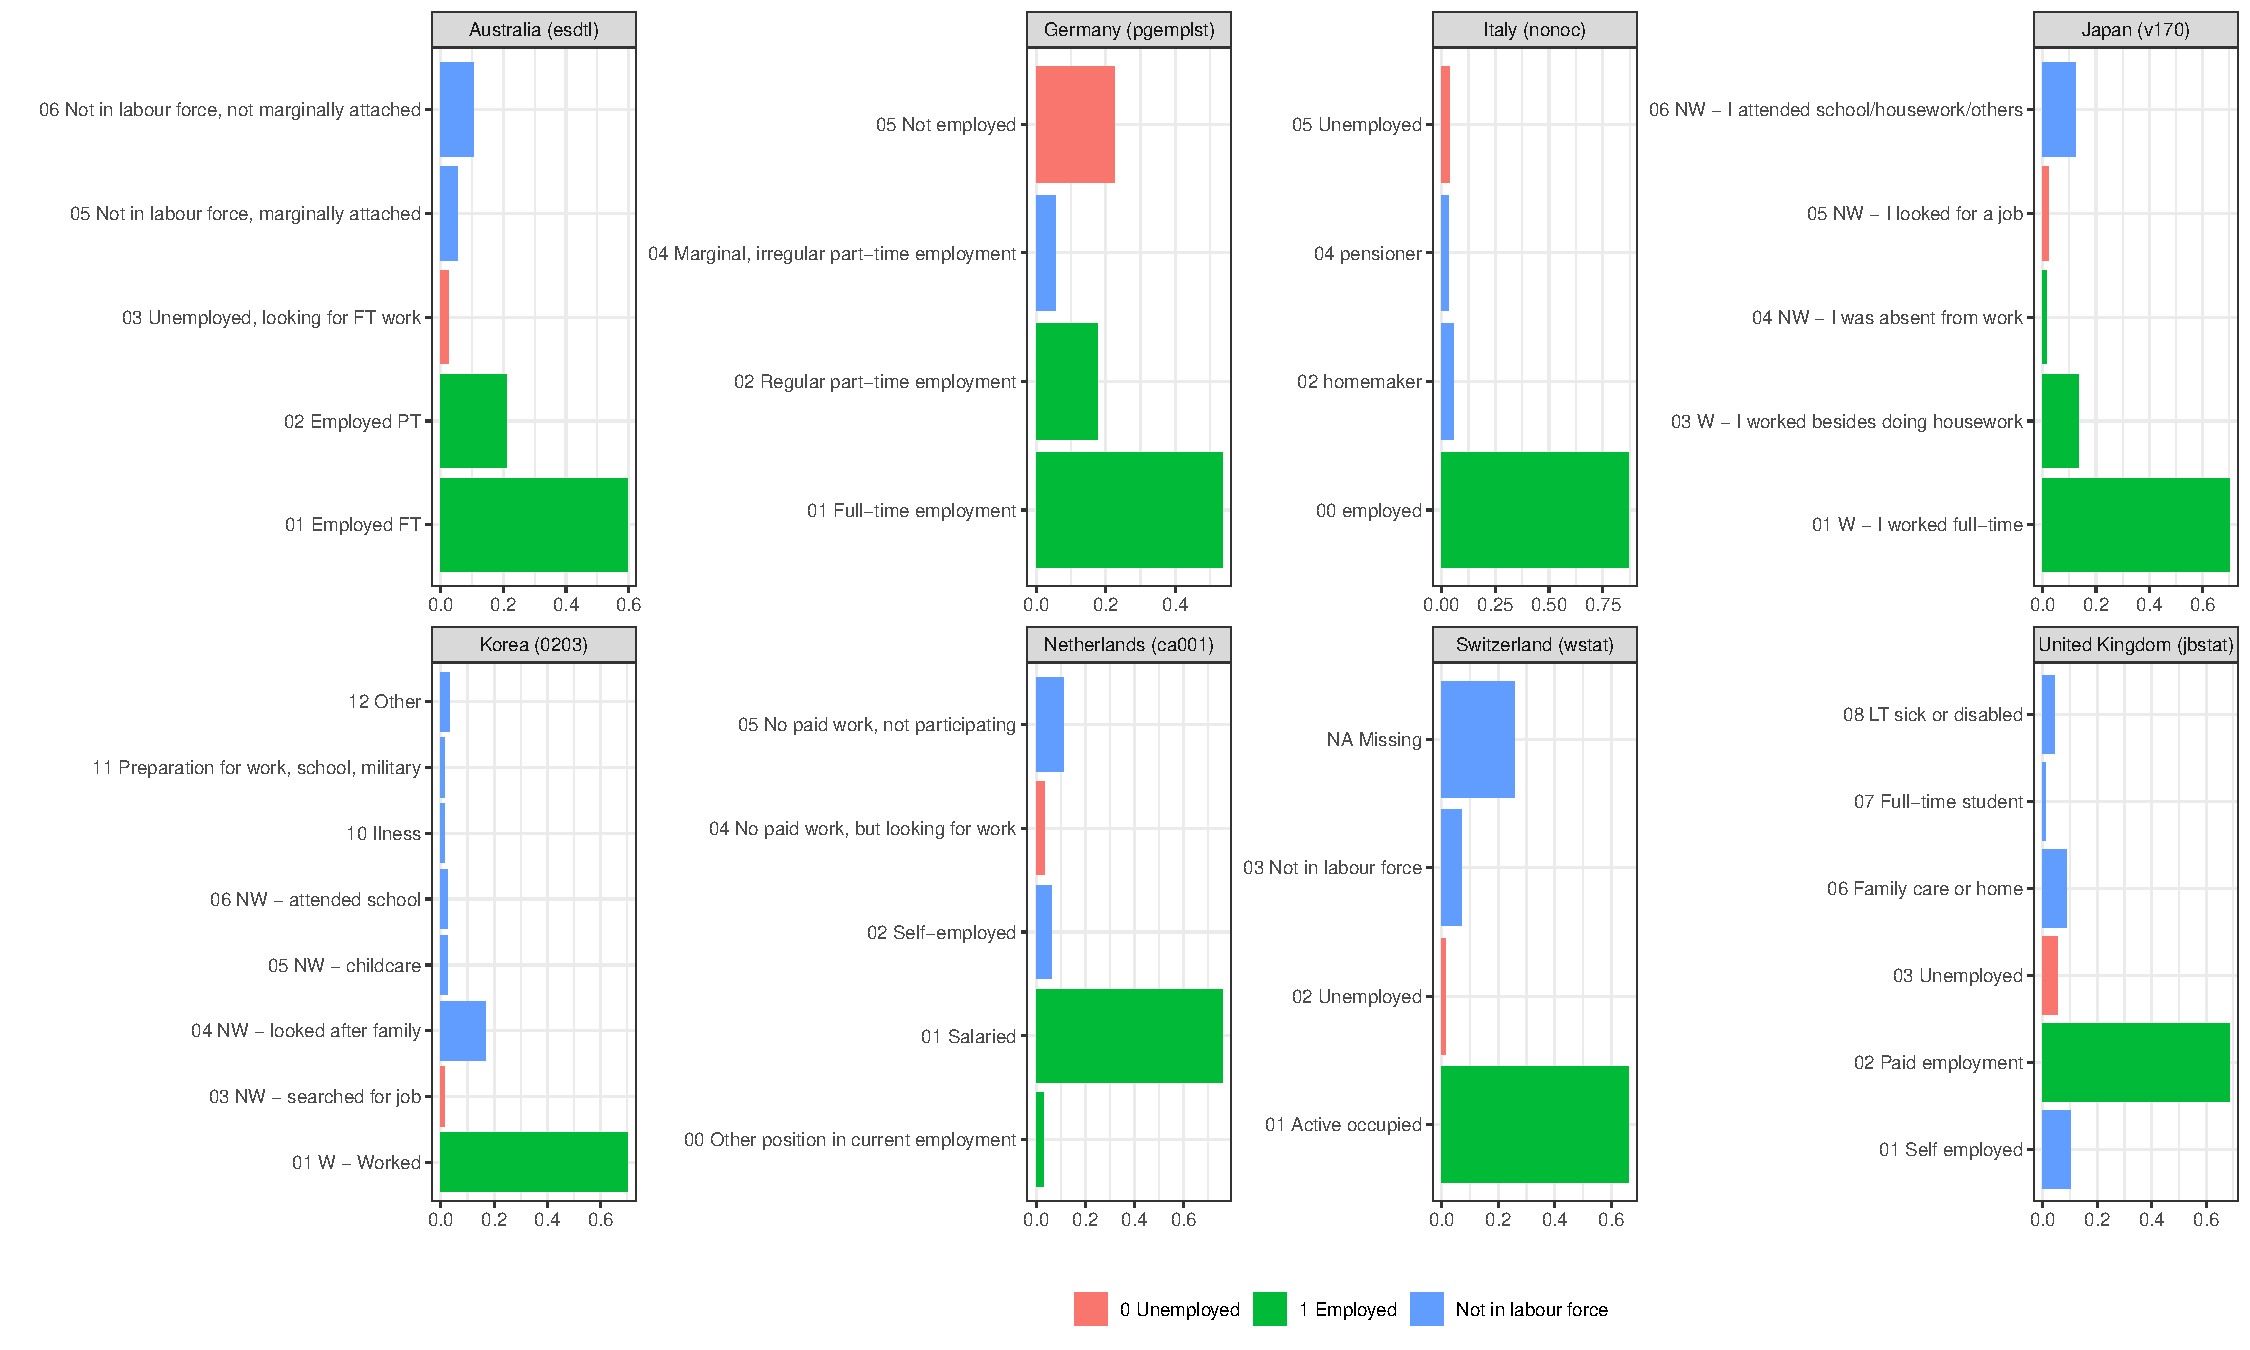
\includegraphics{../../../graphs/descriptives/graph_descriptives_emp_status.pdf}}
    \label{graph_descriptives_emp_status}
\end{sidewaysfigure}

\begin{sidewaysfigure}[h!]
    \caption{Recode contract type by country (conditional on employed with contract)}
    \resizebox{\textwidth}{!}{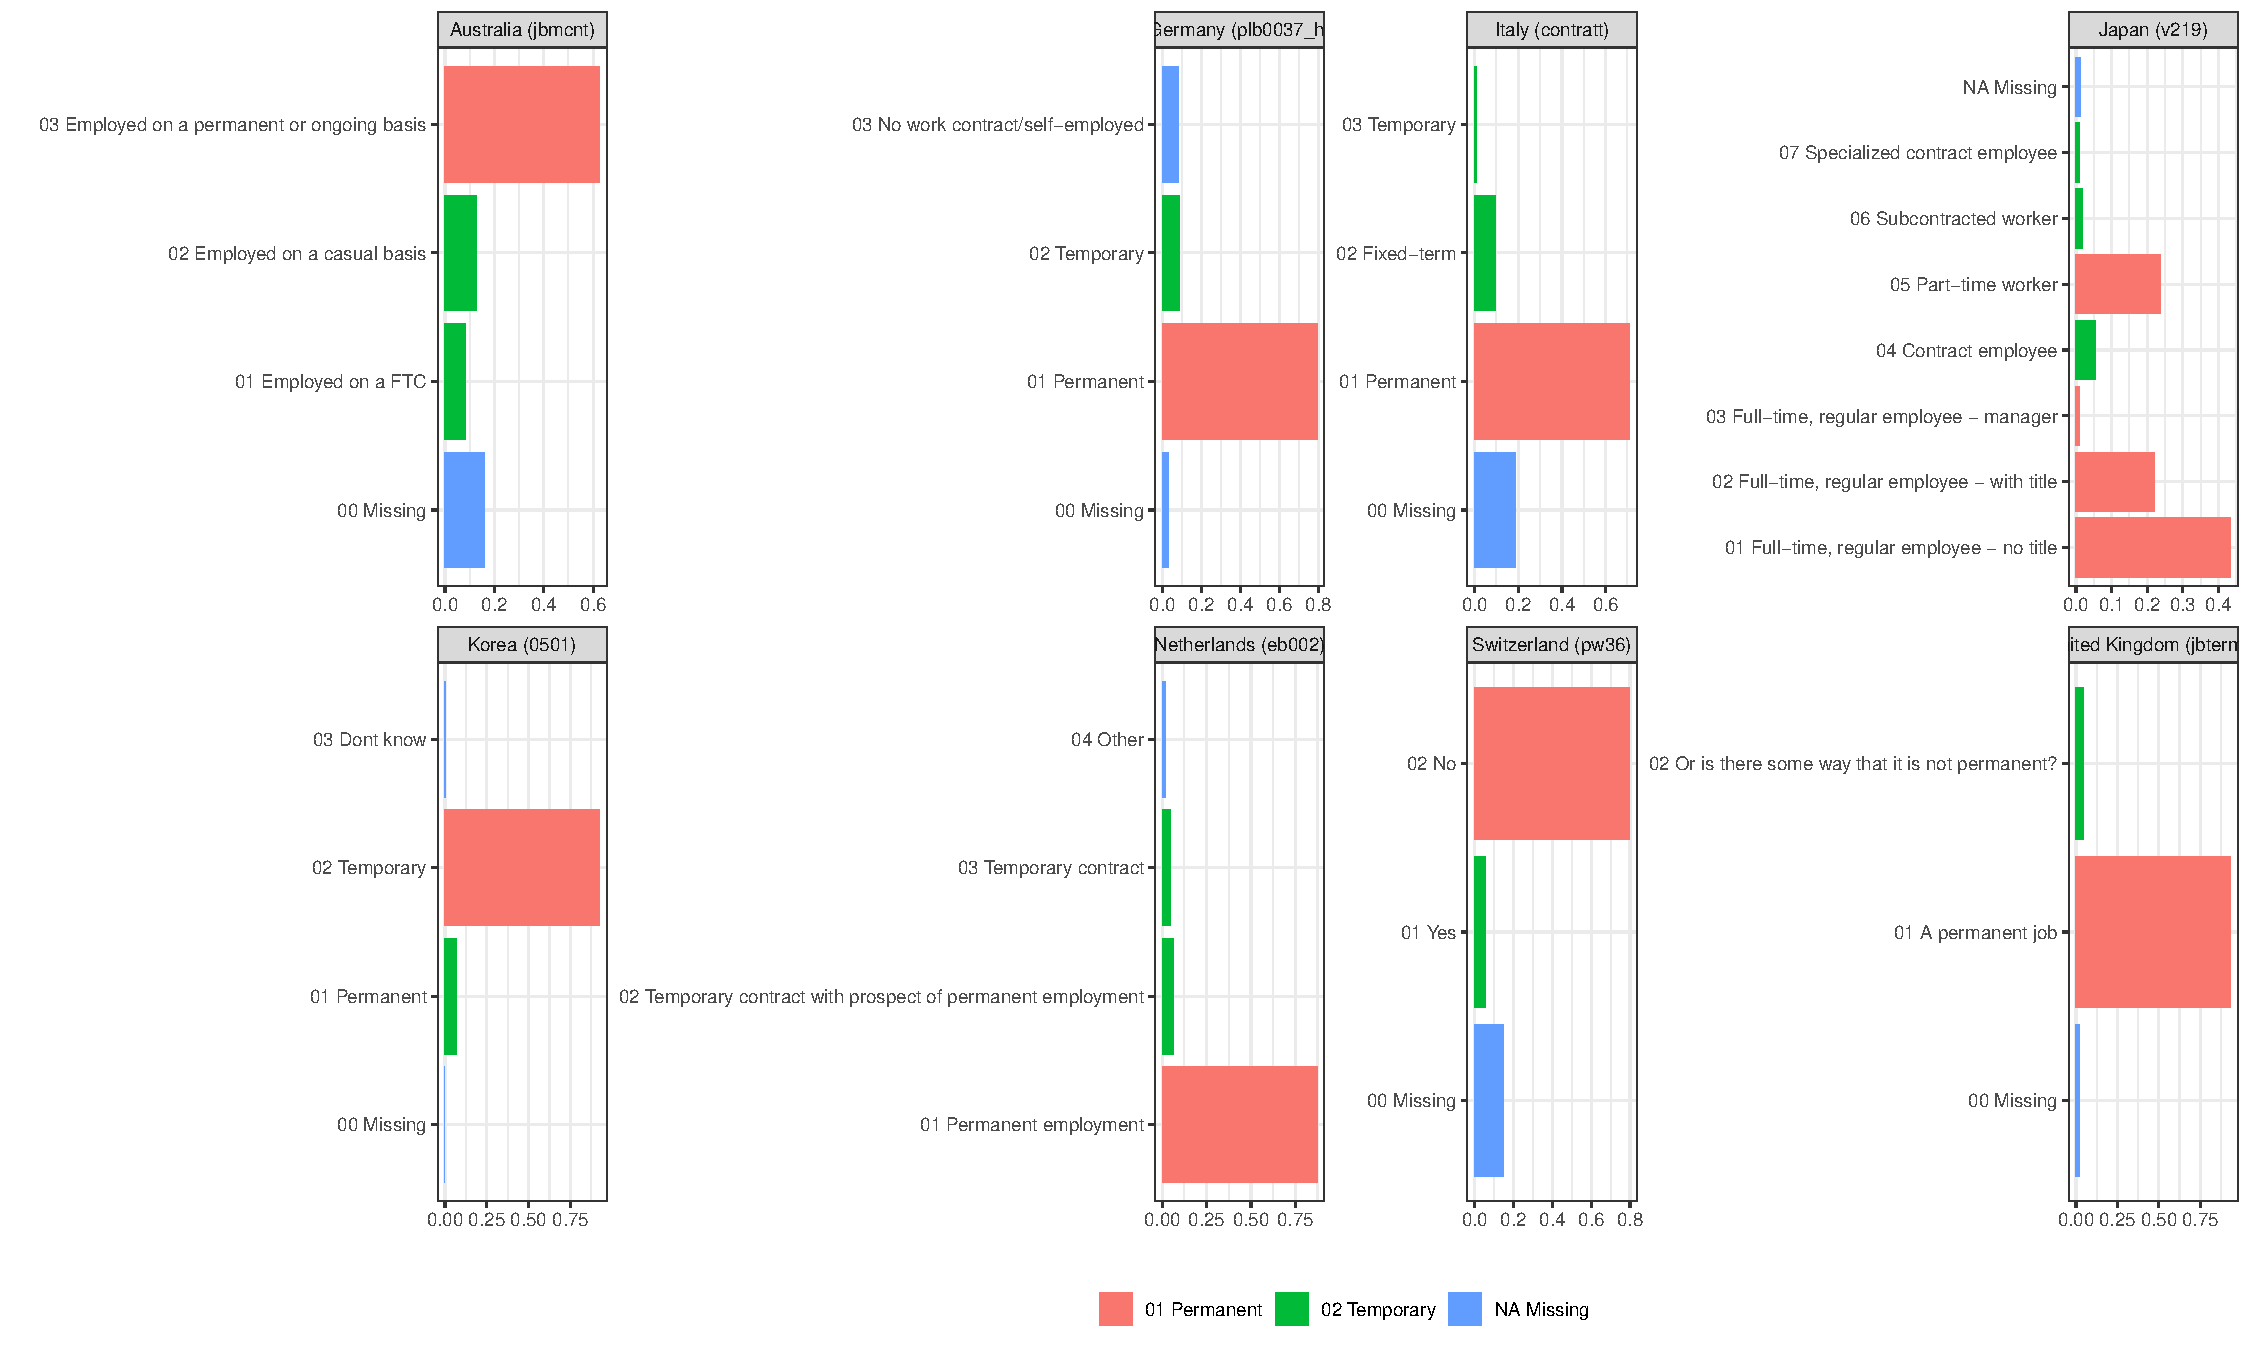
\includegraphics{../../../graphs/descriptives/graph_descriptives_contyp.pdf}}
    \label{graph_descriptives_contyp}
\end{sidewaysfigure}

\begin{sidewaysfigure}[h!]
    \caption{Recode education by country}
    \resizebox{\textwidth}{!}{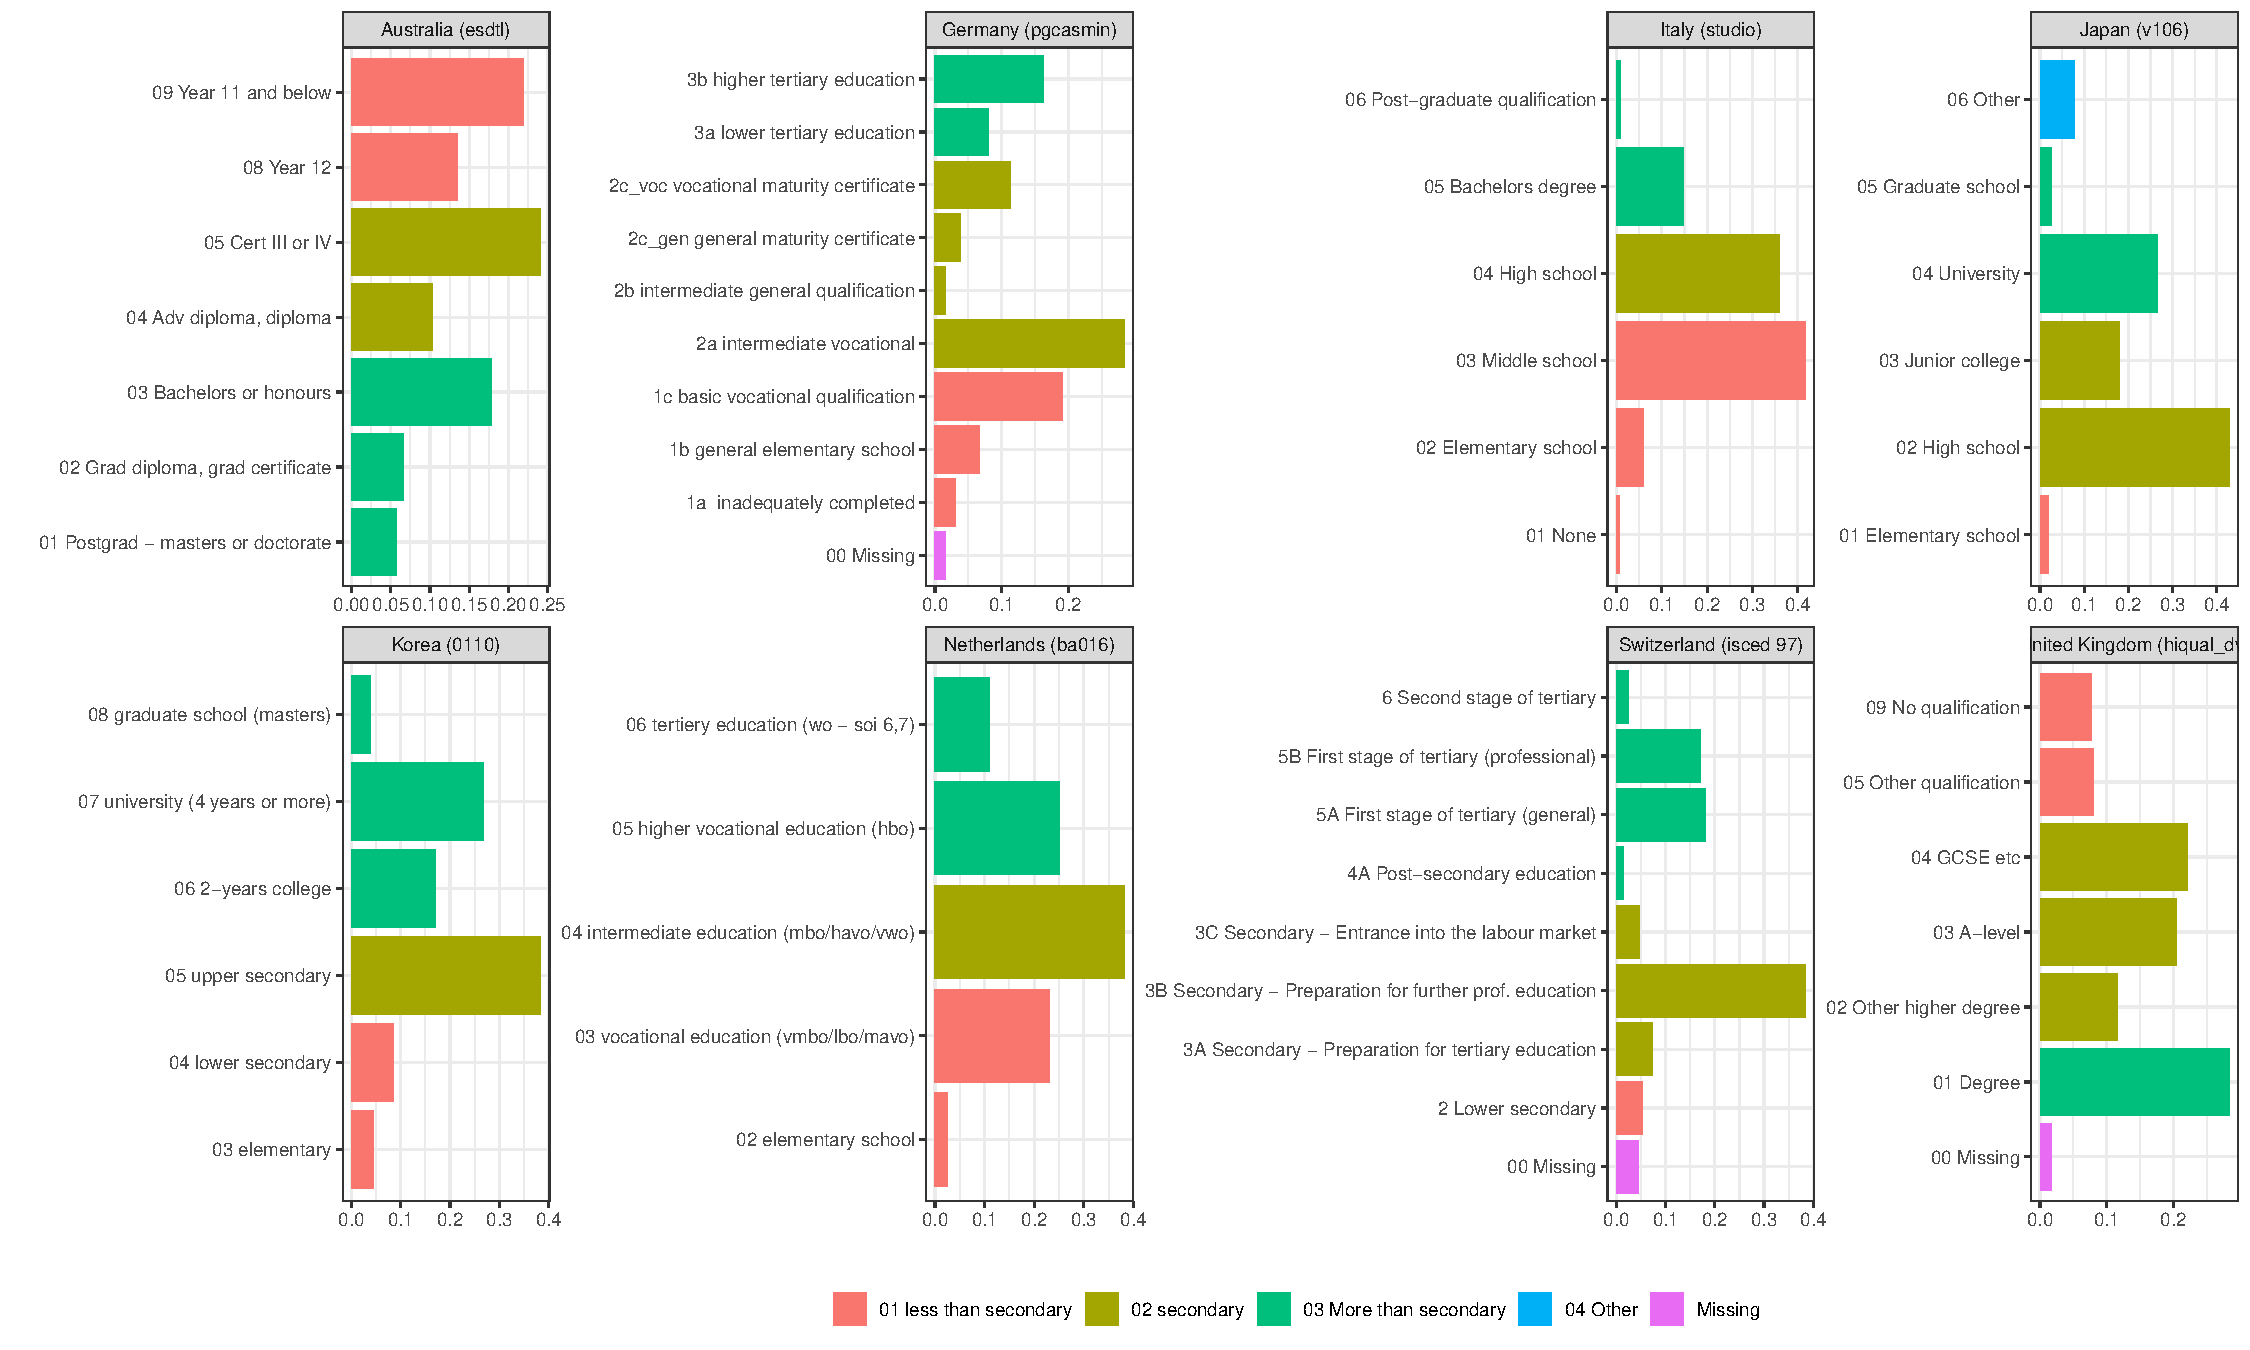
\includegraphics{../../../graphs/descriptives/graph_descriptives_education.pdf}}
    \label{graph_descriptives_education}
\end{sidewaysfigure}


%%%%%%%%%%%%%%%%%%%%%%%%%%%%%%%%%%%%%%%%%%
%%%%%%%%%%%%%%%%%%%%%%%%%%%%%%%%%%%%%%%%%%
%%%%%%%%%%%%%%%%%%%%%%%%%%%%%%%%%%%%%%%%%%
%%%%%%%%%%%%%%%%%%%%%%%%%%%%%%%%%%%%%%%%%%
\clearpage
\section{Appendix: Sample selection}\label{appendix:sample_selection}
\setcounter{figure}{0}    
\setcounter{table}{0}    
\renewcommand*\thetable{\Alph{section}.\arabic{table}}
\renewcommand*\thefigure{\Alph{section}.\arabic{figure}}
\renewcommand{\theHfigure}{\Alph{section}.\arabic{table}}
\renewcommand{\theHtable}{\Alph{section}.\arabic{figure}}

Given concerns of bias resulting from the sample selection criteria that reduced the sample by over 50\% in step 9 of table \ref{table_sample_filter_steps_country}, we compare LN average income, unemployment rate, and temporary employment rate from cross-sectional samples A and B to estimates from the World Bank or OECD.  Figure \ref{graph_descriptives_income_better_paper.pdf} compares cross-sectional annual average income (LN) from Sample B to data from the OECD.  The trends are almost identical.  Figure \ref{graph_descriptives_unmp_paper} compares cross-sectional annual unemployment rate from Sample A data from the World Bank.  Unemployment rate comes from World Bank data, not OECD because OECD does not include Switzerland before 2010, after 2010, both data sources are the same.  The trends are almost identical.  Figure  \ref{graph_descriptives_temp_paper} compares cross-sectional temporary employment rate to data from OECD.  With the exception of Japan and Korea, results are qualitatively similar.

The data covers the time frame from 2000 to 2018.  In order to understand any meaningful changes in legislation within the countries that could affect the relationship between temporary employment and wages, figure \ref{graph_epl} displays changes in employment protection legislation (EPL) for temporary and permanent contracts for the eight countries in our sample \citep[Ch. 3]{oecd2020recent}.  With the exception of Germany and Italy, there is little change in EPL within countries.  In Italy, EPL for temporary contracts declined from 3.25 in 2000 to 2.0 in 2003.  In Germany, EPL for temporary contracts declined from 2.0 in 2000 to 1 in 2004.  Given the general stability in EPL trends, there is little reason to be concerned that the findings presented here can be explained by changes in EPL.

In addition, we provide more detail about the frequency counts of transitions into and out of temporary employment, as shown in table \ref{table_sample_filter_steps_country_transitions}.  In sample B, around 12\% of the sample make a transition from a temporary to a permanent contract, and 9\% make a transition from a permanent to a temporary contract.  In sample A, around 5\% make a transition from unemployment to a permanent contract, and 2\% make a transition from unemployment to a temporary contract. 

Table \ref{table_sample_unmp_steps_contyp} specifies why the number of transitions from unemployment to temporary or permanent employment are so small.  The answer is high panel attrition for individuals who experience unemployment.  In sample A, 18\% experience unemployment.  Of those who experience unemployment, only about 50\% exit into a temporary or permanent contract (8\% of the sample).  Of those who exit unemployment into a contract, 75\% are also employed at least one additional period within 5 years after the transition (6\% of the sample).  The authors note that similar levels of panel attrition exist among those who experience unemployment in the uncleaned, raw data for a sample of prime age workers 25-54 who are either unemployed or working with a contract type (table \ref{descriptives_table_unemployment}).  

Finally, we compare frequency counts from the sample selection criteria for the two data sets from the Netherlands.  The Labour Supply Panel (LSP) is what is used in the paper and the Longitudinal Internet Studies for the Social Sciences is the sensitivity data.  As discussed in Appendix \ref{appendix:data}, there are advantages and disadvantages of the LISS and the LSP, but the LISS suffers from a much greater panel attrition, as shown in table \ref{table_sample_filter_steps_country_NE}.


\begin{sidewaysfigure}[!h]
    \caption{Compare annual average income (LN) from sample to OECD}
    \resizebox{\textwidth}{!}{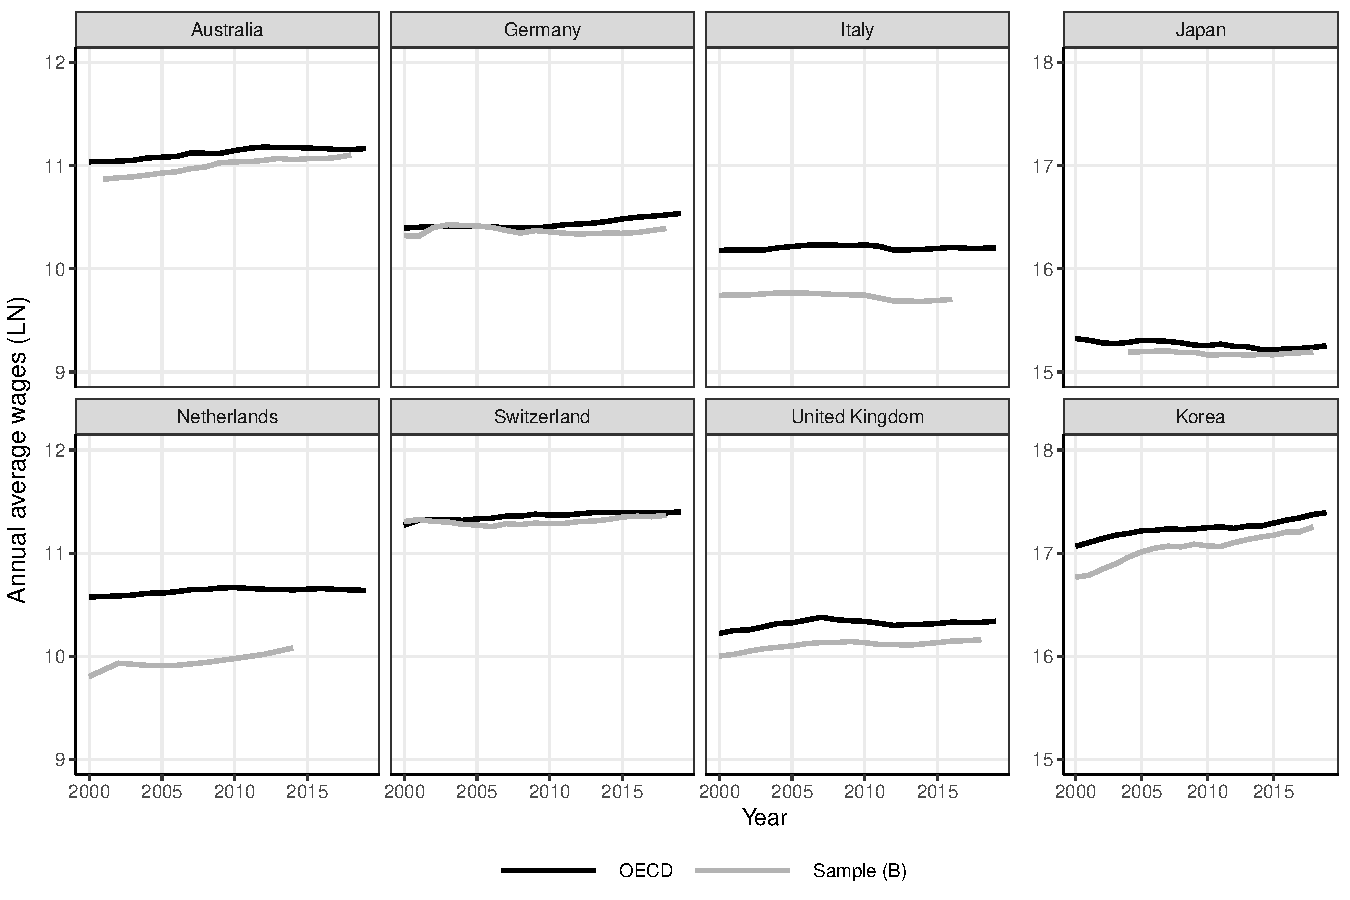
\includegraphics{../../../graphs/descriptives/graph_descriptives_income_better_paper.pdf}}
    \label{graph_descriptives_income_better_paper.pdf}
\end{sidewaysfigure}

\begin{sidewaysfigure}[!h]
    \caption{Compare unemployment rate from sample to World Bank}
    \resizebox{\textwidth}{!}{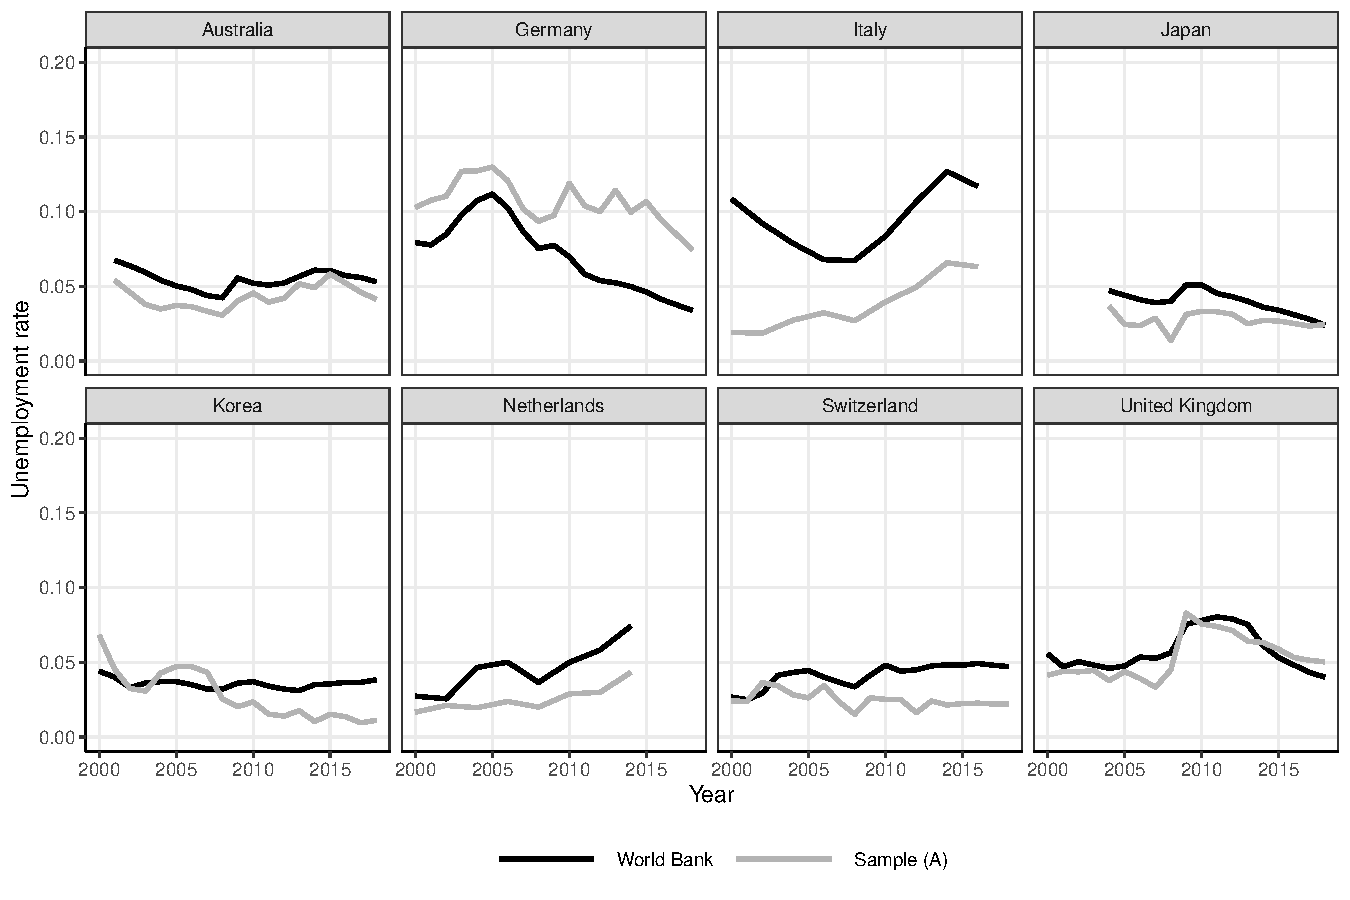
\includegraphics{../../../graphs/descriptives/graph_descriptives_unmp_paper.pdf}}
    \label{graph_descriptives_unmp_paper}
\end{sidewaysfigure}

\begin{sidewaysfigure}[!h]
    \caption{Compare temporary employment rate from sample to OECD}
    \resizebox{\textwidth}{!}{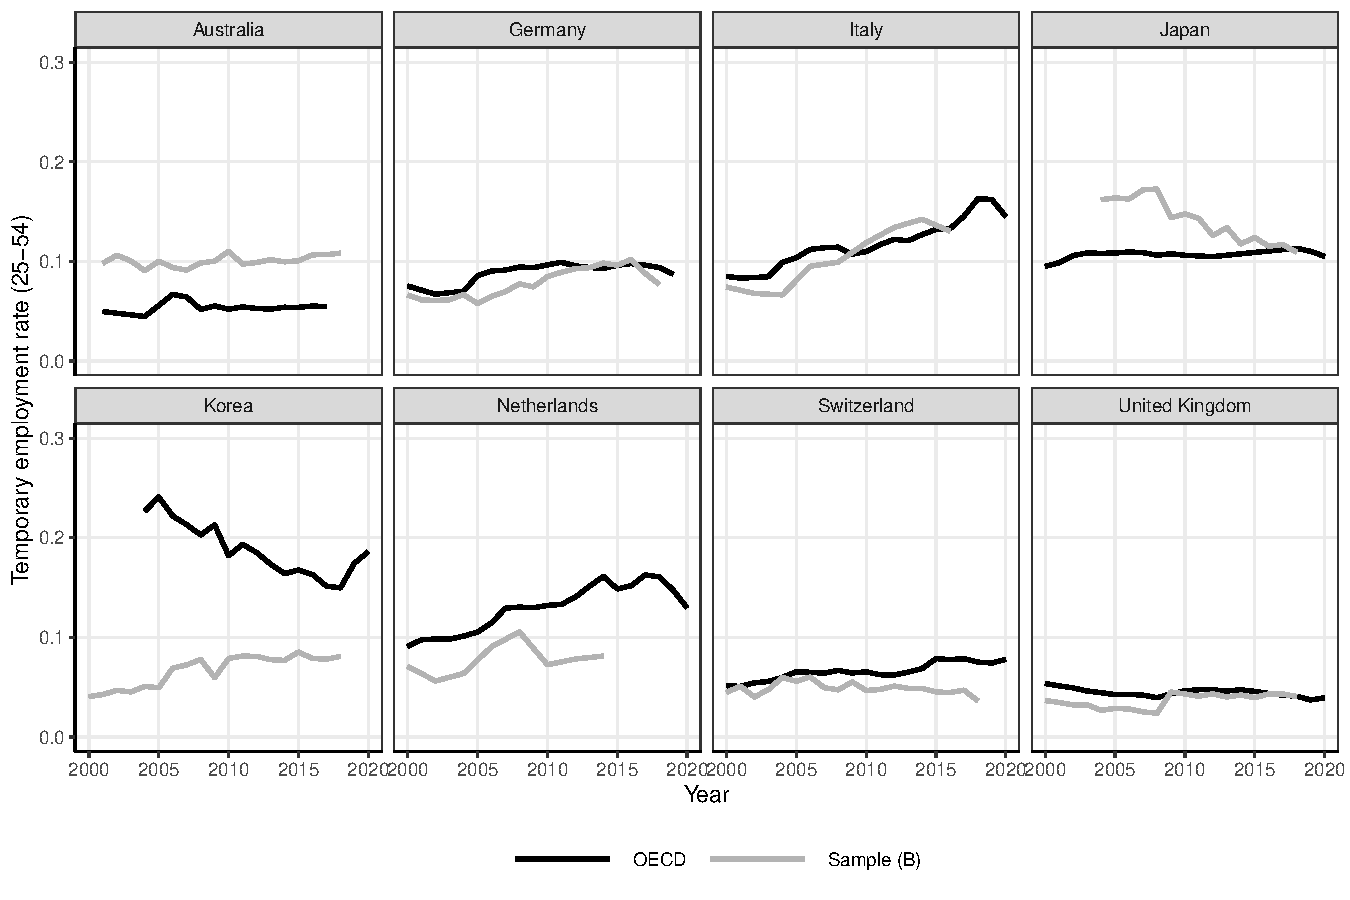
\includegraphics{../../../graphs/descriptives/graph_descriptives_temp_paper.pdf}}
    \label{graph_descriptives_temp_paper}
\end{sidewaysfigure}


\begin{sidewaysfigure}[!h]
    \caption{Changes in employment protection legislation over time (OECD)}
    \resizebox{\textwidth}{!}{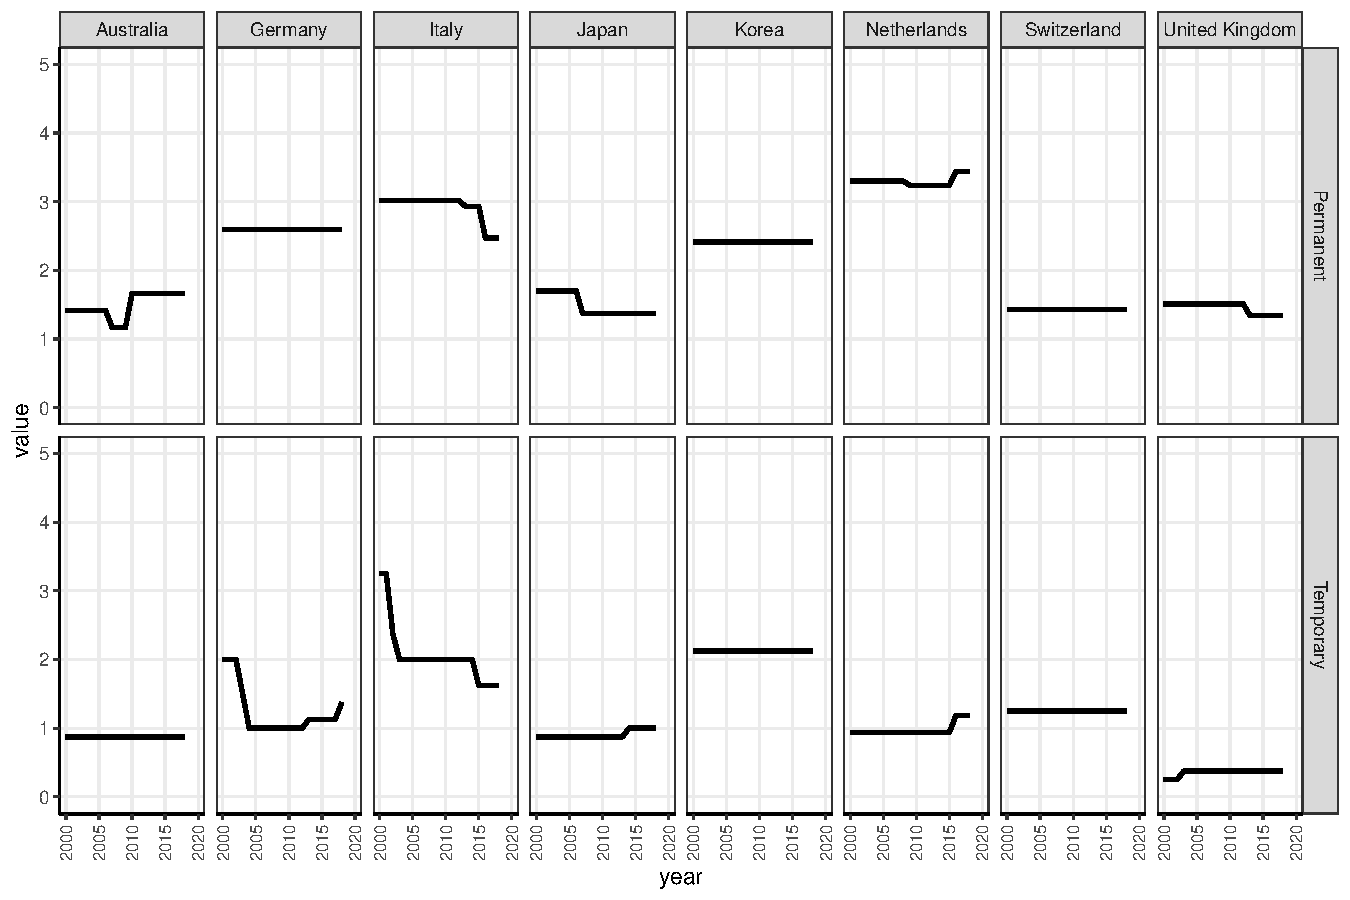
\includegraphics{../../../graphs/descriptives/graph_epl.pdf}}
    \label{graph_epl}
\end{sidewaysfigure}


\begin{sidewaystable}[!h]
    \caption{Country specific frequency and transition counts into and out of temporary employment}
    \centering
    \resizebox{\textwidth}{!}{\begin{tabular}{l>{\raggedright\arraybackslash}p{2.5in}llllllllllllllllll}
   \toprule 
 
\multicolumn{14}{l}{{\bf Panel A:} Sample selection criteria} \\ 

&  & 
\multicolumn{2}{l}{Total (all countries)} &
\multicolumn{2}{l}{Australia} &
\multicolumn{2}{l}{Germany} &
\multicolumn{2}{l}{Italy} &
\multicolumn{2}{l}{Japan} &
\multicolumn{2}{l}{Korea} &
\multicolumn{2}{l}{Netherlands} &
\multicolumn{2}{l}{Switzerland} &
\multicolumn{2}{l}{United Kingdom}
\\  
 
 
\multicolumn{1}{l}{Step} & 
\multicolumn{1}{l}{Description} 
& n & $\Delta$
& n & $\Delta$
& n & $\Delta$
& n & $\Delta$
& n & $\Delta$
& n & $\Delta$
& n & $\Delta$
& n & $\Delta$
& n & $\Delta$
\\ 
\cmidrule(lr){1-2}
\cmidrule(lr){3-4}
\cmidrule(lr){5-6}
\cmidrule(lr){7-8}
\cmidrule(lr){9-10}
\cmidrule(lr){11-12}
\cmidrule(lr){13-14}
\cmidrule(lr){15-16}
\cmidrule(lr){17-18}
\cmidrule(lr){19-20}
\\[-1.8ex]  
 
0 & Raw data & 415,771 &  & 31,951 &  & 91,693 &  & 100,847 &  & 10,499 &  & 24,491 &  & 14,458 &  & 34,469 &  & 107,363 &  \\ 
  1 & Panel years between 2000 and 2018 & 367,032 & -12\% & 31,951 & 0\% & 83,722 & -9\% & 68,012 & -33\% & 10,499 & 0\% & 23,515 & -4\% & 14,458 & 0\% & 34,469 & 0\% & 100,406 & -6\% \\ 
  2 & Prime age (25 - 54) & 210,900 & -43\% & 19,431 & -39\% & 52,198 & -38\% & 33,724 & -50\% & 6,315 & -40\% & 16,089 & -32\% & 9,693 & -33\% & 17,205 & -50\% & 56,245 & -44\% \\ 
  3 & Labour force participant (employed or unemployed) & 157,370 & -25\% & 15,881 & -18\% & 38,538 & -26\% & 25,547 & -24\% & 4,787 & -24\% & 10,980 & -32\% & 7,461 & -23\% & 9,251 & -46\% & 44,925 & -20\% \\ 
  4 & Non missing education or gender & 155,535 & -1\% & 15,875 & 0\% & 37,635 & -2\% & 25,547 & 0\% & 4,767 & 0\% & 10,978 & 0\% & 7,449 & 0\% & 9,251 & 0\% & 44,033 & -2\% \\ 
  5 & Hourly wages within the top/bottom 0.005 percentile & 154,743 & -1\% & 15,817 & 0\% & 37,454 & 0\% & 25,336 & -1\% & 4,754 & 0\% & 10,943 & 0\% & 7,404 & -1\% & 9,168 & -1\% & 43,867 & 0\% \\ 
  6 & Sample A: At least 3 observations & 79,148 & -49\% & 10,598 & -33\% & 20,972 & -44\% & 3,678 & -85\% & 3,179 & -33\% & 7,311 & -33\% & 2,418 & -67\% & 5,303 & -42\% & 25,689 & -41\% \\ 
  7 & Sample B: + always employed & 73,189 & -8\% & 10,072 & -5\% & 18,302 & -13\% & 3,449 & -6\% & 3,079 & -3\% & 7,103 & -3\% & 2,320 & -4\% & 5,153 & -3\% & 23,711 & -8\% \\ 
   
\hline \\[-1.8ex]  
 
\multicolumn{14}{l}{{\bf Panel B:} Data sets by event type (if treated, must be employed after treatment)} \\ 

& 
& \# & \%
& \# & \%
& \# & \%
& \# & \%
& \# & \%
& \# & \%
& \# & \%
& \# & \%
& \# & \%
\\ 
\cmidrule(lr){1-2}
\cmidrule(lr){3-4}
\cmidrule(lr){5-6}
\cmidrule(lr){7-8}
\cmidrule(lr){9-10}
\cmidrule(lr){11-12}
\cmidrule(lr){13-14}
\cmidrule(lr){15-16}
\cmidrule(lr){17-18}
\cmidrule(lr){19-20}
\\[-1.8ex]  
 
A & Unmp $\rightarrow$ perm & 3,670 & 5\% & 452 & 4\% & 1,036 & 5\% & 48 & 1\% & 155 & 5\% & 382 & 5\% & 21 & 1\% & 167 & 3\% & 1,409 & 5\% \\ 
  A & Unmp $\rightarrow$ temp & 1,268 & 2\% & 148 & 1\% & 623 & 3\% & 41 & 1\% & 34 & 1\% & 40 & 1\% & 36 & 1\% & 35 & 1\% & 311 & 1\% \\ 
  B & Temp $\rightarrow$ perm & 9,063 & 12\% & 2,270 & 23\% & 2,757 & 15\% & 291 & 8\% & 227 & 7\% & 893 & 13\% & 260 & 11\% & 360 & 7\% & 2,005 & 8\% \\ 
  B & Perm $\rightarrow$ temp & 6,800 & 9\% & 1,992 & 20\% & 1,559 & 9\% & 237 & 7\% & 232 & 8\% & 822 & 12\% & 198 & 9\% & 250 & 5\% & 1,510 & 6\% \\ 
   \bottomrule \\[-1.8ex] \multicolumn{20}{p{12in}}{Note: n - is unique observations.  $\Delta$ - is difference in n from previous step.  \# - is unique n who experienced at least 1 event.  \% - is percent who experienced an event.} 
\end{tabular}
}
    \label{table_sample_filter_steps_country_transitions}
\end{sidewaystable}

\begin{sidewaystable}[!h]
    \caption{Why are the number of unemployment exits so small in table \ref{table_sample_filter_steps_country_transitions}?}
    \centering
    \resizebox{\textwidth}{!}{\begin{tabular}{l>{\raggedright\arraybackslash}p{2in}llllllllllllllllll}
   \\[-1.8ex]\hline\hline \\ 
 [-1.8ex]
\multicolumn{20}{l}{{\bf Panel A:} Sample selection criteria} \\ 

&  & 
\multicolumn{2}{l}{Total (all countries)} &
\multicolumn{2}{l}{Australia} &
\multicolumn{2}{l}{Germany} &
\multicolumn{2}{l}{Italy} &
\multicolumn{2}{l}{Japan} &
\multicolumn{2}{l}{Korea} &
\multicolumn{2}{l}{Netherlands} &
\multicolumn{2}{l}{Switzerland} &
\multicolumn{2}{l}{United Kingdom}
\\  
 
 
\multicolumn{1}{l}{Step} & 
\multicolumn{1}{l}{Description} 
& n & $\Delta$
& n & $\Delta$
& n & $\Delta$
& n & $\Delta$
& n & $\Delta$
& n & $\Delta$
& n & $\Delta$
& n & $\Delta$
& n & $\Delta$
\\ 
\cmidrule(lr){1-2}
\cmidrule(lr){3-4}
\cmidrule(lr){5-6}
\cmidrule(lr){7-8}
\cmidrule(lr){9-10}
\cmidrule(lr){11-12}
\cmidrule(lr){13-14}
\cmidrule(lr){15-16}
\cmidrule(lr){17-18}
\cmidrule(lr){19-20}
\\[-1.8ex]  
 
1 & Total unemployment events (From data set A) & 14,450 &  & 1,917 &  & 5,562 &  & 335 &  & 364 &  & 980 &  & 184 &  & 531 &  & 4,577 &  \\ 
  2 & Must exit unemployment & 6,463 & -55\% & 1,060 & -45\% & 2,079 & -63\% & 145 & -57\% & 212 & -42\% & 478 & -51\% & 90 & -51\% & 256 & -52\% & 2,143 & -53\% \\ 
  3 & Employed at least 1 period after exit (within 5 years) & 4,847 & -25\% & 592 & -44\% & 1,608 & -23\% & 86 & -41\% & 184 & -13\% & 419 & -12\% & 56 & -38\% & 199 & -22\% & 1,703 & -21\% \\ 
   
\hline \\[-1.8ex]  
 
\multicolumn{20}{l}{{\bf Panel B:} Frequency, by event type} \\ 

& 
&  \# & \%
&  \# & \%
&  \# & \%
&  \# & \%
&  \# & \%
&  \# & \%
&  \# & \%
&  \# & \%
&  \# & \%
\\ 
\cmidrule(lr){1-2}
\cmidrule(lr){3-4}
\cmidrule(lr){5-6}
\cmidrule(lr){7-8}
\cmidrule(lr){9-10}
\cmidrule(lr){11-12}
\cmidrule(lr){13-14}
\cmidrule(lr){15-16}
\cmidrule(lr){17-18}
\cmidrule(lr){19-20}
\\[-1.8ex]  
 
 & Unmp $\rightarrow$ temp & 1,268 & 26\% & 148 & 25\% & 623 & 39\% & 41 & 48\% & 34 & 18\% & 40 & 10\% & 36 & 64\% & 35 & 18\% & 311 & 18\% \\ 
   & Unmp $\rightarrow$ perm & 3,670 & 76\% & 452 & 76\% & 1,036 & 64\% & 48 & 56\% & 155 & 84\% & 382 & 91\% & 21 & 38\% & 167 & 84\% & 1,409 & 83\% \\ 
   & U $\rightarrow$ P \& U $\rightarrow$ T & 91 &  & 8 &  & 51 &  & 3 &  & 5 &  & 3 &  & 1 &  & 3 &  & 17 &  \\ 
   \hline \\[-1.8ex] \multicolumn{20}{p{12in}}{Notes: n - is unique observations.  
               $\Delta$ - is difference in n from previous step.  
               \# - is number of transitions.  
               \% - is percent of total transitions from step 3. 
               \% is more than 100\% because some individuals experience both a transition from Unmp to Perm and Unmp to Temp.} 
\end{tabular}
}
    \label{table_sample_unmp_steps_contyp}
\end{sidewaystable}

\begin{sidewaystable}[!h]
    \caption{Panel attrition for individuals who experience unemployment}
    \centering
    \resizebox{\textwidth}{!}{\begin{tabular}{llllllllllllllllll}
   \toprule 
 
&&
\multicolumn{2}{l}{Australia} &
\multicolumn{2}{l}{Germany} &
\multicolumn{2}{l}{Italy} &
\multicolumn{2}{l}{Japan} &
\multicolumn{2}{l}{Korea} &
\multicolumn{2}{l}{Netherlands} &
\multicolumn{2}{l}{Switzerland} &
\multicolumn{2}{l}{United Kingdom}
\\  
 
 
\multicolumn{1}{l}{Periods} & 
\multicolumn{1}{l}{Description} 
& n & $\Delta$
& n & $\Delta$
& n & $\Delta$
& n & $\Delta$
& n & $\Delta$
& n & $\Delta$
& n & $\Delta$
& n & $\Delta$
\\ 
\cmidrule(lr){1-2}
\cmidrule(lr){3-4}
\cmidrule(lr){5-6}
\cmidrule(lr){7-8}
\cmidrule(lr){9-10}
\cmidrule(lr){11-12}
\cmidrule(lr){13-14}
\cmidrule(lr){15-16}
\cmidrule(lr){17-18}
\\[-1.8ex]  
 
 & Total observations & 16,260 &  & 41,396 &  & 25,784 &  & 5,075 &  & 11,610 &  & 8,082 &  & 10,745 &  & 46,395 &  \\ 
  1 period & Ever unemployed & 2,950 & -82\% & 11,274 & -73\% & 1,311 & -95\% & 542 & -89\% & 1,547 & -87\% & 695 & -91\% & 894 & -92\% & 8,422 & -82\% \\ 
  2 periods & + Exit unemployment & 1,442 & -51\% & 3,442 & -69\% & 166 & -87\% & 288 & -47\% & 686 & -56\% & 174 & -75\% & 460 & -49\% & 2,457 & -71\% \\ 
  3 periods & + 1 period after exit & 1,137 & -21\% & 2,338 & -32\% & 69 & -58\% & 236 & -18\% & 572 & -17\% & 78 & -55\% & 342 & -26\% & 1,771 & -28\% \\ 
   \bottomrule  
\end{tabular}
}
    \label{descriptives_table_unemployment}
\end{sidewaystable}


\begin{table}[!h]
    \caption{Sample filter steps comparing LISS and LSP from the Netherlands}
    \centering
    \resizebox{\textwidth}{!}{\begin{tabular}{llllll}
   \toprule 
 [-1.8ex]
\multicolumn{6}{l}{{\bf Panel A:} Sample selection criteria} \\ 

&  & 
\multicolumn{2}{l}{NE - LSP} &
\multicolumn{2}{l}{NE - LISS}
\\  
 
 
\multicolumn{1}{l}{Step} & 
\multicolumn{1}{l}{Description} 
& n & $\Delta$
& n & $\Delta$
\\ 
\cmidrule(lr){1-2}
\cmidrule(lr){3-4}
\cmidrule(lr){5-6}
\\[-1.8ex]  
 
0 & Raw data & 14,458 &  & 13,121 &  \\ 
  1 & Panel years between 2000 and 2018 & 14,458 & 0\% & 12,976 & -1\% \\ 
  2 & Prime age (25 - 54) & 9,693 & -33\% & 6,641 & -49\% \\ 
  3 & Labour force participant (employed or unemployed) & 8,757 & -10\% & 5,505 & -17\% \\ 
  4 & Unemployed or employed with contract type & 8,082 & -8\% & 4,981 & -10\% \\ 
  5 & Unemployed or employed with wages & 7,765 & -4\% & 3,814 & -23\% \\ 
  6 & Unemployed or employed with monthly hours between 40 and 320 & 7,461 & -4\% & 3,758 & -1\% \\ 
  7 & Non missing education or gender & 7,449 & 0\% & 3,746 & 0\% \\ 
  8 & Hourly wages within the top/bottom 0.005 percentile & 7,404 & -1\% & 3,720 & -1\% \\ 
  9 & Sample A: At least 3 observations & 2,418 & -67\% & 1,432 & -62\% \\ 
  10 & Sample B: + always employed & 2,325 & -4\% & 1,313 & -8\% \\ 
   
\hline \\[-1.8ex]  
 
\multicolumn{6}{l}{{\bf Panel B:} Data sets by event type (if treated, must be employed after treatment)} \\ 

& 
& \# & \%
& \# & \%
\\ 
\cmidrule(lr){3-4}
\cmidrule(lr){5-6}
\\[-1.8ex]  
 
A & Unmp $\rightarrow$ perm & 19 & 1\% & 12 & 1\% \\ 
  A & Unmp $\rightarrow$ temp & 32 & 1\% & 8 & 1\% \\ 
  B & Temp $\rightarrow$ perm & 174 & 7\% & 63 & 5\% \\ 
  B & Perm $\rightarrow$ temp & 182 & 8\% & 44 & 3\% \\ 
   \bottomrule \\[-1.8ex] \multicolumn{6}{p{7in}}{Notes: In Panel A: n - is unique observations and $\Delta$ - is difference in n from previous step.  In Panel B: \# - is unique n who experienced at least 1 event and \% - is percent who experienced an event.} 
\end{tabular}
}
    \label{table_sample_filter_steps_country_NE}
\end{table}

%%%%%%%%%%%%%%%%%%%%%%%%%%%%%%%%%%%%%%%%%%
%%%%%%%%%%%%%%%%%%%%%%%%%%%%%%%%%%%%%%%%%%
%%%%%%%%%%%%%%%%%%%%%%%%%%%%%%%%%%%%%%%%%%
%%%%%%%%%%%%%%%%%%%%%%%%%%%%%%%%%%%%%%%%%%
\clearpage
\section{Appendix: Multiple events}\label{appendix:multiple}
\setcounter{figure}{0}    
\setcounter{table}{0}    
\renewcommand*\thetable{\Alph{section}.\arabic{table}}
\renewcommand*\thefigure{\Alph{section}.\arabic{figure}}
\renewcommand{\theHfigure}{\Alph{section}.\arabic{table}}
\renewcommand{\theHtable}{\Alph{section}.\arabic{figure}}

Let us imagine employment status for one individual in 6 periods of time looks like this: T (50) $\rightarrow$ P (90) $\rightarrow$T (110) $\rightarrow$ P (130) $\rightarrow$ T (140) $\rightarrow$ T (150), as shown in table \ref{table_compare_transformed_data_original} and figure \ref{graph_descriptives_multiple_events_num}.  In this case, we observe four distinct events T $\rightarrow$ P ($\times 2$), and P $\rightarrow$ T ($\times 2$).  

\begin{itemize} 
    \item T $\rightarrow$ P ($\times 2$)
    \begin{itemize} 
        \item $\hat{\beta} event^{T \rightarrow P (1)}_{it} = 40$ 
        \item $\hat{\beta} event^{T \rightarrow P (2)}_{it} = 20$
        \item The average of the two events: $\hat{\beta} event^{T \rightarrow P}_{it} = 30$
    \end{itemize}
    \item P $\rightarrow$ T ($\times 2$)
    \begin{itemize} 
        \item $\hat{\beta} event^{P \rightarrow T (1)}_{it} = 20$
        \item $\hat{\beta} event^{P \rightarrow T (2)}_{it} = 10$
        \item The average of the two events: $\hat{\beta} event^{P \rightarrow T}_{it} = 15$
    \end{itemize}
\end{itemize}

In order to model each of the four distinct events, we must transform the data from person, year data into person, event, year data.  The steps are as follows:

\begin{enumerate}  
    \item For each individual, filter one row per individual, transition at the year the transition occurs ($t_0$).  The result is four rows, one for each event.  This is data frame $A$.
    \item Create 3 variables in data frame $A$:
    \begin{enumerate}
        \item $eventyear=year$ is the year the transition took place  
        \item $transeq$ is cumulative to identify each individual, transition
        \item $eventtime=0$ is for period the transition took place
    \end{enumerate}  
    \item Create data frame $B$ by selecting five variables: $pid$, $year$, $transseq$, $eventyear$, and $eventtime$, i.e. drop $wages$.  
    \item For each individual, transition ($transseq$), we append rows for $eventtime$ four years before ($-$) and six years after the transition ($+$).  Recode $year=year+eventtime$  
    \item Create data frame $C$ by merging data frame $B$ with $A$, by $pid$, $year$ 
    \item In data frame $C$, create a new identifier for each individual, transition sequence ($pidseq$) by multiplying $pid \times transseq \times 100$.  We multiply by 100 to ensure no duplicate $pidseq$
    \item We code the pre/post timing of the distinct events ($event\_p\_t\_time$ and $event\_t\_p\_time$) and create a positive value by adding 3 ($event\_p\_t\_time\_pos$ and $event\_t\_p\_time\_pos$)
\end{enumerate}  

The result is a new data frame with 24 rows: six observations per transition, as shown in table \ref{table_compare_transformed_data_transformed}.  Though not shown, the final steps in the process are to transform the $eventtime\_pos$ for each distinct transition into dummies (reference is year before event, i.e. 2).  

The transformed data do not alter the findings obtained by applying FE and FEIS models to untransformed data, as shown in table \ref{table_compare_transformed_data_original}.  As in the paper, we note that while there are alternative solutions to modeling both transitions simultaneously.  For example, Allison \citeyearpar{allison_asymmetric_2019} codes a transition from one status to another as a permanent and absorbing event.  While this solution is appropriate for some types of events, this is not an appropriate solution for employment status, which changes over time.  However, as shown in figure \ref{graph_sensitivity_single_multiple_events}, if we followed the Allison solution, estimates from first, single event are similar to estimates from multiple events.  The reason is that most people do not experience multiple events of the same transition, but some do, as shown in figure \ref{graph_descriptives_multiple_events_num}.  


\begin{lstlisting}[language=R]
# Create empty work space

rm(list=ls())

# Load library 

library(tidyverse)

# Step 1: Create data 

df_a <- data.frame(
        pid = c(1,1,1,1,1,1),
        year = c(1,2,3,4,5,6),
        wage = c(50,90,110,130,140,150),
        temp = c(1,0,1,0,1,1),
        perm = c(0,1,0,1,0,0)
)

# Step 2: Identify transitions 

df_b <- df_a %>%
        arrange(pid, year) %>%
        group_by(pid) %>%
        # identify type of transition
        mutate(event_t_p_yes = ifelse(perm == 1 & lag(temp,1) == 1 & row_number()>1, yes = 1, no = NA),
               event_p_t_yes = ifelse(temp == 1 & lag(perm,1) == 1 & row_number()>1, yes = 1, no = NA),
        ) %>%
        ungroup() %>%
        # identify whether trans is whether transition occurred
        mutate(trans = rowSums(select(., contains("event_")), na.rm = TRUE)) %>%
        group_by(pid) %>%
        # transseq is the cumulative count for number of transitions
        mutate(transseq = cumsum(ifelse(is.na(trans), 0, trans))) %>%
        ungroup()

# Step 3: Create new data set, 1 row for each transition at time of transition.  

df_c <- df_b %>%
        filter(trans==1) %>%
        group_by(pid,transseq) %>%
        filter(row_number()==1) %>%
        # identify year transition took place
        mutate(eventtime=0,
               eventyear=year) %>%
        ungroup() %>%
        select(pid, year, transseq, matches("event"))

# Step 4: Generate sequence indicator for years pre/post transition 

df_d <- data.frame()
event <- c(-4,-3,-2,-1,1,2,3,4,5,6)
for (e in event) {
        df_test <- df_c %>%
                # create eventtime for years pre/post transition
                mutate(eventtime=e) 
        df_d <- rbind(df_d,df_test)
}                

# Step 5: Append data frame from step 2 and 3

df_e <- rbind(df_c,df_d) %>%
        arrange(pid,transseq,eventtime) %>%
        mutate(year = year+eventtime) %>% 
        arrange(pid,transseq,year)

# Step 6: Merge wage data

df_f <- merge(df_e,df_a) %>%
        arrange(pid,transseq,year) %>%
        mutate(pidseq=pid*100+transseq) %>%  # new identifier
        select(pid, year, pidseq, transseq, wage, temp, perm, eventyear, eventtime, everything())


# Step 7: Code events

df_g <- df_f %>%
  arrange(pidseq,year) %>%
  group_by(pidseq) %>%
  # temp to perm
  mutate(event_t_p_time = ifelse(event_t_p_yes == 1, yes = year - eventyear, no = 0),
         event_t_p_time = ifelse(event_t_p_time < -2, yes = -3, # lower bound
                                 ifelse(event_t_p_time >= 5, yes = 5, no = event_t_p_time)), # upper bound
         event_t_p_time_pos = ifelse(event_t_p_yes == 1, yes = event_t_p_time + 3, no = 0), # make positive
  ) %>%
  # perm to temp
  mutate(event_p_t_time = ifelse(event_p_t_yes == 1, yes = year - eventyear, no = 0),
         event_p_t_time = ifelse(event_p_t_time < -2, yes = -3, # lower bound
                                 ifelse(event_p_t_time >= 5, yes = 5, no = event_p_t_time)), # upper bound
         event_p_t_time_pos = ifelse(event_p_t_yes == 1, yes = event_p_t_time + 3, no = 0), # make positive
  ) %>%
  replace(is.na(.), 0) %>% 
  ungroup()

# Print original and final data frame
print(df_a)

print(df_g)
\end{lstlisting}


\clearpage

\begin{sidewaysfigure}[!h]
    \caption{Simulation figure: Single individual with multiple events}
    \resizebox{\textwidth}{!}{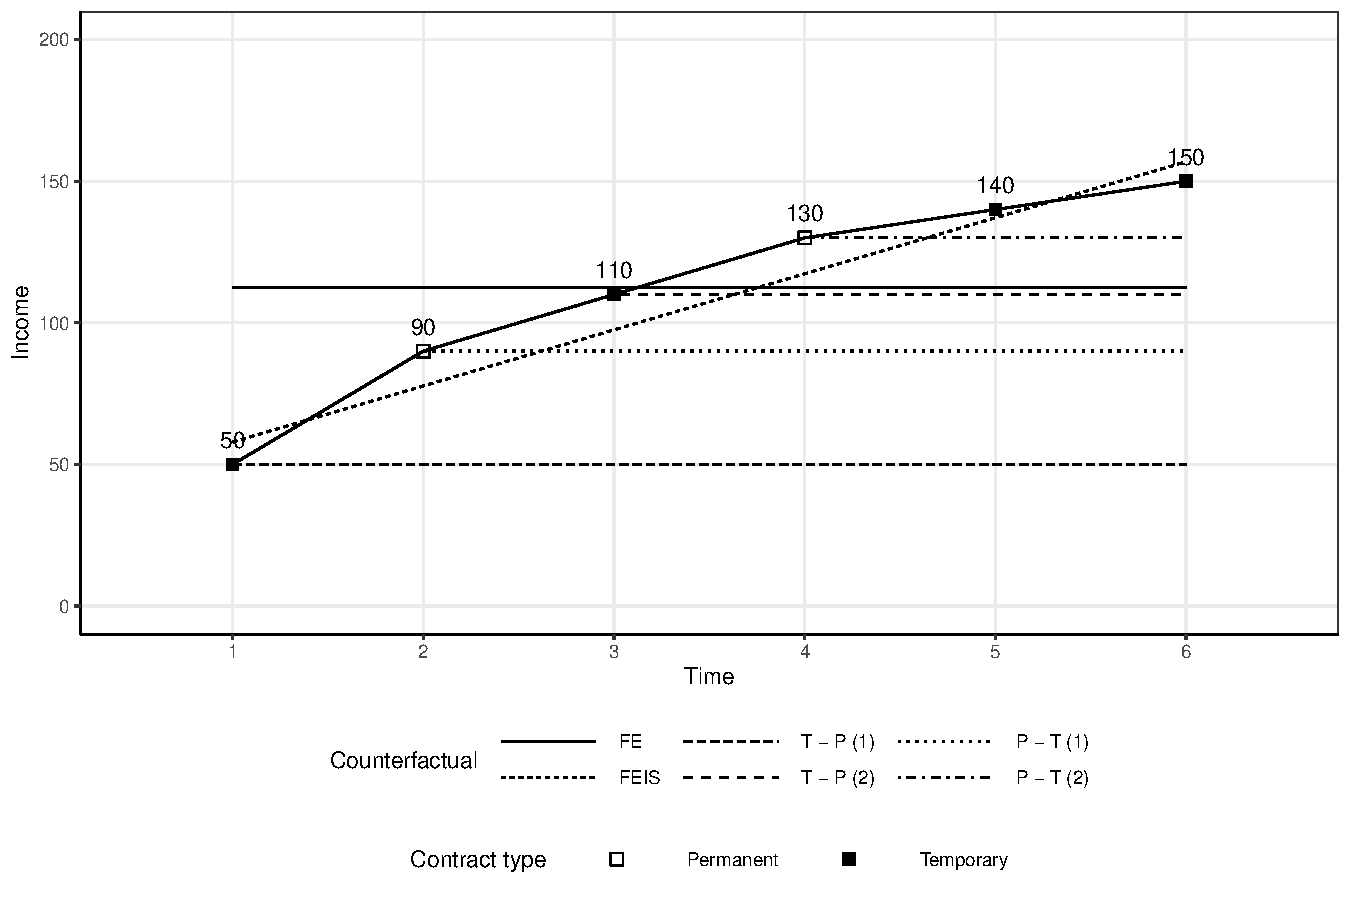
\includegraphics{../../../support_files/simulation/graphs/graph_compare_transformed_data_paper.pdf}}
    \label{graph_compare_transformed_data}
\end{sidewaysfigure}


\begin{table}[!h]
\rowcolors{2}{gray!50}{gray!10}
\caption{Simulation data: Single individual with multiple events}
\centering
    \begin{tabular}{rrrrr}
  \hline
pid & year & temp & perm & wage \\ 
  \hline
1 & 1 & 1 & 0 & 50 \\ 
  1 & 2 & 0 & 1 & 90 \\ 
  1 & 3 & 1 & 0 & 110 \\ 
  1 & 4 & 0 & 1 & 130 \\ 
  1 & 5 & 1 & 0 & 140 \\ 
  1 & 6 & 1 & 0 & 150 \\ 
   \hline
\end{tabular}

\label{table_compare_transformed_data_original}
\end{table}

\begin{table}[!h]
\rowcolors{2}{gray!50}{gray!10}
\caption{Simulation data: Transformed data}
\centering
    \resizebox{\textwidth}{!}{\begin{tabular}{rrrrrrrrrrrr}
  \hline
pid & year & transseq & temp & perm & wage & eventyear & eventtime & event\_p\_t\_yes & event\_t\_p\_yes & event\_p\_t\_time\_pos & event\_t\_p\_time\_pos \\ 
  \hline
1 & 1 & 1 & 1 & 0 & 50 & 2 & -1 & 0 & 1 & 0 & 2 \\ 
  1 & 2 & 1 & 0 & 1 & 90 & 2 & 0 & 0 & 1 & 0 & 3 \\ 
  1 & 3 & 1 & 1 & 0 & 110 & 2 & 1 & 0 & 1 & 0 & 4 \\ 
  1 & 4 & 1 & 0 & 1 & 130 & 2 & 2 & 0 & 1 & 0 & 5 \\ 
  1 & 5 & 1 & 1 & 0 & 140 & 2 & 3 & 0 & 1 & 0 & 6 \\ 
  1 & 6 & 1 & 1 & 0 & 150 & 2 & 4 & 0 & 1 & 0 & 7 \\ 
  1 & 1 & 2 & 1 & 0 & 50 & 3 & -2 & 1 & 0 & 1 & 0 \\ 
  1 & 2 & 2 & 0 & 1 & 90 & 3 & -1 & 1 & 0 & 2 & 0 \\ 
  1 & 3 & 2 & 1 & 0 & 110 & 3 & 0 & 1 & 0 & 3 & 0 \\ 
  1 & 4 & 2 & 0 & 1 & 130 & 3 & 1 & 1 & 0 & 4 & 0 \\ 
  1 & 5 & 2 & 1 & 0 & 140 & 3 & 2 & 1 & 0 & 5 & 0 \\ 
  1 & 6 & 2 & 1 & 0 & 150 & 3 & 3 & 1 & 0 & 6 & 0 \\ 
  1 & 1 & 3 & 1 & 0 & 50 & 4 & -3 & 0 & 1 & 0 & 0 \\ 
  1 & 2 & 3 & 0 & 1 & 90 & 4 & -2 & 0 & 1 & 0 & 1 \\ 
  1 & 3 & 3 & 1 & 0 & 110 & 4 & -1 & 0 & 1 & 0 & 2 \\ 
  1 & 4 & 3 & 0 & 1 & 130 & 4 & 0 & 0 & 1 & 0 & 3 \\ 
  1 & 5 & 3 & 1 & 0 & 140 & 4 & 1 & 0 & 1 & 0 & 4 \\ 
  1 & 6 & 3 & 1 & 0 & 150 & 4 & 2 & 0 & 1 & 0 & 5 \\ 
  1 & 1 & 4 & 1 & 0 & 50 & 5 & -4 & 1 & 0 & 0 & 0 \\ 
  1 & 2 & 4 & 0 & 1 & 90 & 5 & -3 & 1 & 0 & 0 & 0 \\ 
  1 & 3 & 4 & 1 & 0 & 110 & 5 & -2 & 1 & 0 & 1 & 0 \\ 
  1 & 4 & 4 & 0 & 1 & 130 & 5 & -1 & 1 & 0 & 2 & 0 \\ 
  1 & 5 & 4 & 1 & 0 & 140 & 5 & 0 & 1 & 0 & 3 & 0 \\ 
  1 & 6 & 4 & 1 & 0 & 150 & 5 & 1 & 1 & 0 & 4 & 0 \\ 
   \hline
\end{tabular}
}
\label{table_compare_transformed_data_transformed}
\end{table}

\begin{table}[!h]
    \caption{Parameter estimates using data in table \ref{table_compare_transformed_data_original}, as shown in figure \ref{graph_compare_transformed_data}}
    \centering
    \resizebox{\textwidth}{!}{
\begin{tabular}{l c c c c c c c}
\toprule
 & \multicolumn{2}{c}{FE} & \multicolumn{2}{c}{FEIS} & \multicolumn{3}{c}{FE + IF} \\
\cmidrule(lr){2-3} \cmidrule(lr){4-5} \cmidrule(lr){6-8}
 & Original & Transformed & Original & Transformed & First & First & Multiple \\
\midrule
Temp                     & $2.50$ & $2.50^{***}$ & $-12.39$ & $-12.39^{***}$ &         &         &             \\
                         & $$     & $(0.00)$     & $()$     & $(0.00)$       &         &         &             \\
Event: T $\rightarrow$ P &        &              &          &                & $40.00$ &         & $30.00^{*}$ \\
                         &        &              &          &                & $()$    &         & $(12.38)$   \\
Event: P $\rightarrow$ T &        &              &          &                &         & $20.00$ & $15.00^{*}$ \\
                         &        &              &          &                &         & $()$    & $(6.19)$    \\
\midrule
Num. obs.                & $6$    & $24$         & $6$      & $24$           & $6$     & $6$     & $24$        \\
\bottomrule
\multicolumn{8}{l}{\scriptsize{$^{***}p<0.001$; $^{**}p<0.01$; $^{*}p<0.05$. Note: In FE + IF, pre and post event coefficients are not shown.}}
\end{tabular}
}
    \label{table_compare_transformed_data_output}
\end{table}

\begin{sidewaysfigure}[!h]
    \caption{How many individuals experience multiple events?}
    \resizebox{\textwidth}{!}{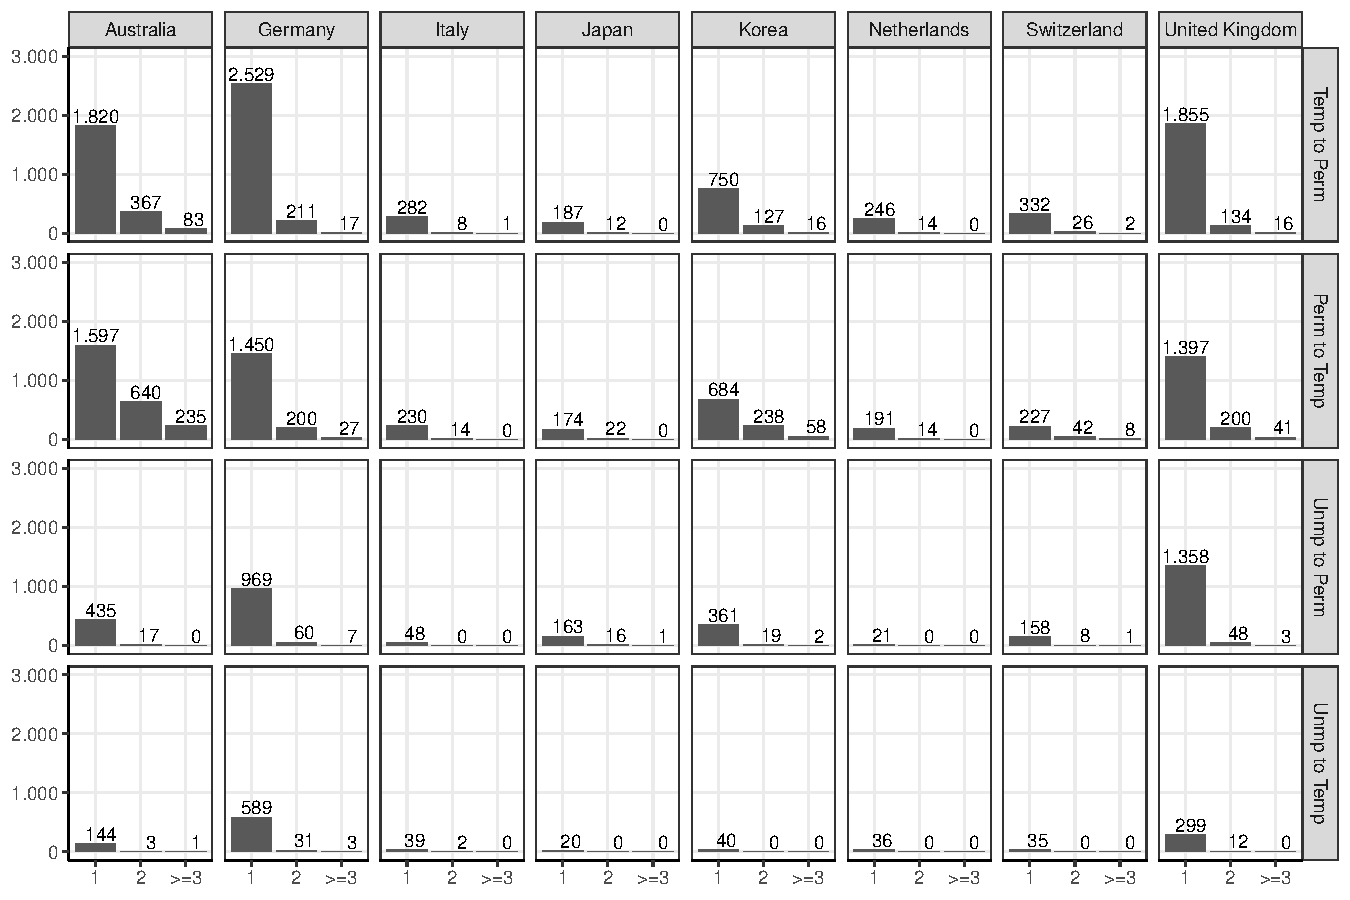
\includegraphics{../../../graphs/descriptives/graph_descriptives_multiple_events_num.pdf}}
    \label{graph_descriptives_multiple_events_num}
\end{sidewaysfigure}

%%%%%%%%%%%%%%%%%%%%%%%%%%%%%%%%%%%%%%%%%%
%%%%%%%%%%%%%%%%%%%%%%%%%%%%%%%%%%%%%%%%%%
%%%%%%%%%%%%%%%%%%%%%%%%%%%%%%%%%%%%%%%%%%
%%%%%%%%%%%%%%%%%%%%%%%%%%%%%%%%%%%%%%%%%%
\clearpage
\section{Appendix: Simulation exercise}\label{appendix:simulation}
\setcounter{figure}{0}    
\setcounter{table}{0}    
\renewcommand*\thetable{\Alph{section}.\arabic{table}}
\renewcommand*\thefigure{\Alph{section}.\arabic{figure}}
\renewcommand{\theHfigure}{\Alph{section}.\arabic{table}}
\renewcommand{\theHtable}{\Alph{section}.\arabic{figure}}

To illustrate our methodological approach, we describe three simple simulations with two individuals in six periods of time, as shown in figure \ref{graph_compare_models_simulation_paper}. In simulation 1, both individuals are the same age and live in the same country. Individual A begins period 1 with a temporary contract earning €100. Individual B begins period 1 with a permanent contract earning €300. In period 4, both individuals switch contracts. Individual A transitions from a temporary to a permanent contract, increasing their wages by €30, to €130. By contrast, individual B transitions from a permanent to a temporary contract, reducing their wages by €30, to €270. Individual-specific counterfactual wages are average wages in a temporary contract. In simulation 1, a temporary contract pays €30 less compared to a permanent contract and -30 is the effect of a temporary contract on wages.

When we apply the FE model \ref{eq:model_fe} to simulation 1, the $\beta$ coefficient for temporary employment is -30, which is the correct effect of a temporary contract on wages, as shown in table \ref{table_compare_models_simulation_paper}.\footnote{$-30 = \frac{(\text{Ind. A} + \text{Ind. B}) \cdot (\text{Avg. wages in Temp} - \text{Avg. wages in Perm})}{2 \text{ individuals}} = \frac{(270-300) + (100-130)}{2} = \frac{(-30) + (-30)}{2} = \frac{-60}{2}$}

Next, let us build on this simulation to include non-parallel trends.  In simulation 2, we assume that individual A, who transitions from a temporary to a permanent contract has a higher wage trajectory, than individual B, who transitions from a permanent to a temporary contract.  The only difference between simulation 1 and simulation 2 is that individual A increases their wages by €20 in each period of time.  Individual B's wages do not change.

Despite the distinct wage trajectories, a temporary contract still pays €30 less than a counterfactual permanent contract assuming trends remained the same.  Therefore, just as in simulation 1, the effect of a temporary contract on wages is still -30.  However, as shown in table 2, when we apply the FE model to simulation 2, the $\beta$  coefficient for temporary employment is -60,\footnote{$-60 = \frac{(\text{Ind. A} + \text{Ind. B}) \cdot (\text{Avg. wages in Temp} - \text{Avg. wages in Perm})}{2 \text{ individuals}} = \frac{(120-210) + (270-300)}{2} = \frac{(-90) + (-30)}{2} = \frac{-120}{2}$} which incorrectly identifies that the effect of a temporary contract on wages because it does not account for the distinct wage trajectories of the two individuals.  

To account for non-parallel trends, we extend model \ref{eq:model_fe} into a random trend model by adding individual-specific linear outcome trends, i.e. interaction terms between a continuous variable for age with the fixed effect for individual ($\alpha_i age_{it}$).  This is referred to as a fixed effects individual slopes (FEIS) estimator  \citep{ludwig_is_2018}, as shown in model \ref{eq:model_feis}.  Data are detrended by subtracting estimated individual linear trend for each variable. This eliminates both individual heterogeneity in levels ($\alpha_i$) and slopes ($\alpha_i age_{it}$). Hence, the FEIS estimator rests on a weaker exogeneity assumption than the FE estimator as it allows for confounding by time-constant variables that lead to linear trends in the outcome variable. When we apply the FEIS estimator to simulation 1 or 2, the $\beta$ coefficient for temporary employment is -30, which is the average difference between actual and counterfactual wages if trends remained the same. 

% The methodological approach used in model \ref{eq:model_feis} follows Brüderl and Ludwig \citeyearpar{ludwig_is_2018}, who cite Wooldridge \citeyearpar[pp. 377–81]{wooldridge_econometric_2010}, but FEIS also has a rich history in the literature examining the consequences of unemployment \citep{jacobson_earnings_1993,stevens_persistent_1997}. 

The issue is that neither the FE nor FEIS models correctly distinguish between asymmetric effect of two distinct events: the positive effect of a transition from temporary into permanent (T $\rightarrow$ P) and the negative effect of a transition from permanent into temporary (P $\rightarrow$ T).  Standard FE estimators must not be interpreted according to the estimation equation, but in line with the structural model that defines the wage effect of having a temporary versus permanent contract \citep{an_causal_2017,wooldridge_econometric_2010}.   The problem is that standard FE models are agnostic with respect to the direction and timing of the transition. Instead, standard FE models only compares average wages when an individual has a temporary contract relative to average wages when that same individual has a permanent contract.  This is still true in standard FEIS models, even if FEIS models do control for differences in individual slopes. 

When we apply the AFE + DIF model \ref{eq:model_afe_temp} to simulation 2, the $\beta$ coefficient for the event T $\rightarrow$ P in period 4 is +50 and the comparable $\beta$ coefficient for the event P $\rightarrow$ T is -30.  The AFE + DIF model classifies the effect of a given transition as the raw, or unadjusted difference in wages between period 4, the year the transition takes place, and period 3, the year before.   

Therefore, unlike the FEIS model \ref{eq:model_feis}, the FE + DIF model  \ref{eq:model_afe_temp} does account for the asymmetric effect of the two events.  The FE + DIF also controls for individual-specific wage trends, but not in the same way as FEIS.  While FEIS assumes that a wage trend's slope or direction is the linear parameter for individual slopes, AFE + DIF makes no assumptions about a wage trend's slope or direction.  We see this as an advantage.  


\begin{sidewaysfigure}[!h]
    \caption{Simulation data}
    \resizebox{\textwidth}{!}{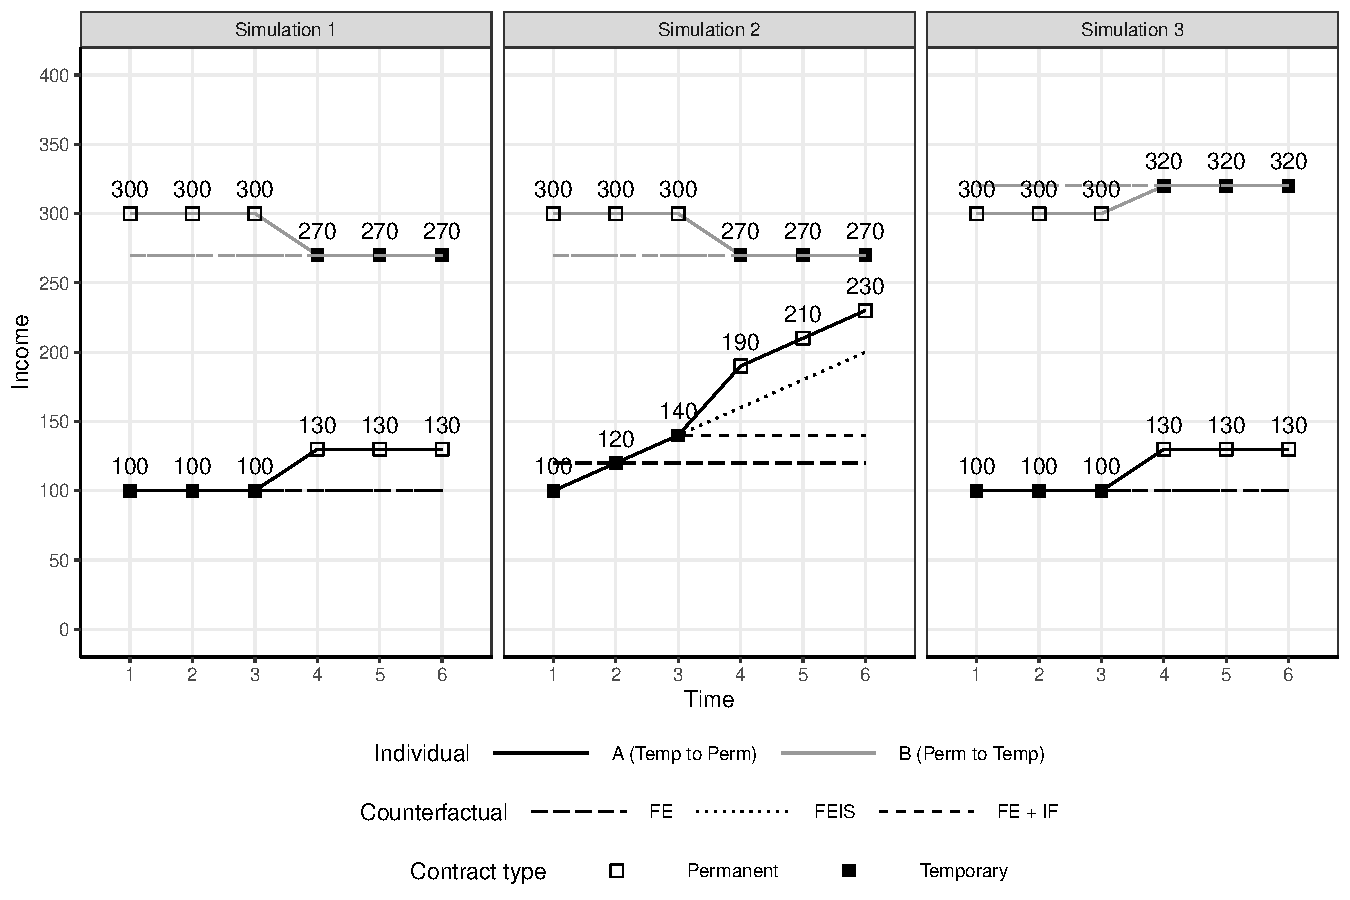
\includegraphics{../../../support_files/simulation/graphs/graph_compare_models_simulation_paper.pdf}}
    \label{graph_compare_models_simulation_paper}
\end{sidewaysfigure}

\begin{table}[!h]
    \caption{Parameter estimates}
    \centering
    \resizebox{\textwidth}{!}{
\begin{tabular}{l c c c c c c c c c}
\toprule
 & \multicolumn{3}{c}{Simulation 1} & \multicolumn{3}{c}{Simulation 2} & \multicolumn{3}{c}{Simulation 3} \\
\cmidrule(lr){2-4} \cmidrule(lr){5-7} \cmidrule(lr){8-10}
 & FE & FEIS & AFE + DIF & FE & FEIS & AFE + DIF & FE & FEIS & AFE + DIF \\
\midrule
Temp                     & $-30.00^{***}$ & $-30.00^{***}$ &          & $-60.00$  & $-30.00^{***}$ &          & $-5.00$   & $-5.00$   &          \\
                         & $(0.00)$       & $(0.00)$       &          & $(31.46)$ & $(0.00)$       &          & $(26.22)$ & $(27.64)$ &          \\
Event: T $\rightarrow$ P &                &                & $30.00$  &           &                & $50.00$  &           &           & $30.00$  \\
                         &                &                & $(0.00)$ &           &                & $(0.00)$ &           &           & $(0.00)$ \\
Event: P $\rightarrow$ T &                &                & $-30.00$ &           &                & $-30.00$ &           &           & $20.00$  \\
                         &                &                & $(0.00)$ &           &                & $(0.00)$ &           &           & $(0.00)$ \\
\bottomrule
\multicolumn{10}{l}{\scriptsize{$^{***}p<0.001$; $^{**}p<0.01$; $^{*}p<0.05$. Note: In AFE + DIF, pre and post event coefficients are not shown.}}
\end{tabular}
}
    \label{table_compare_models_simulation_paper}
\end{table}


%%%%%%%%%%%%%%%%%%%%%%%%%%%%%%%%%%%%%%%%%%
%%%%%%%%%%%%%%%%%%%%%%%%%%%%%%%%%%%%%%%%%%
%%%%%%%%%%%%%%%%%%%%%%%%%%%%%%%%%%%%%%%%%%
%%%%%%%%%%%%%%%%%%%%%%%%%%%%%%%%%%%%%%%%%%
\clearpage
\section{Appendix: Raw coefficients}\label{appendix:coefficients}
\setcounter{table}{0}
\setcounter{figure}{0}
\renewcommand*\thetable{\Alph{section}.\arabic{table}}
\renewcommand*\thefigure{\Alph{section}.\arabic{figure}}
\renewcommand{\theHfigure}{\Alph{section}.\arabic{table}}
\renewcommand{\theHtable}{\Alph{section}.\arabic{figure}}

In this appendix section, we provide the estimated coefficients, standard errors and 95\% confidence intervals for figures \ref{graph_contyp} and \ref{graph_unmp}.

\begin{table}[!h]
    \caption{Results from standard fixed effects (FE) model \ref{eq:model_fe} in figure \ref{graph_contyp}}
    \centering
    \begin{tabular}{lrrrr}
   \toprule 
 
country & estimate & std.error & ymin & ymax \\ 

\cmidrule(lr){1-5} 
 
\\[-1.8ex]  
 
Australia & -0.0305 & 0.0055 & -0.0412 & -0.0198 \\ 
  Switzerland & -0.0913 & 0.0126 & -0.1160 & -0.0667 \\ 
  Germany & -0.0779 & 0.0056 & -0.0888 & -0.0670 \\ 
  Japan & -0.0405 & 0.0213 & -0.0822 & 0.0012 \\ 
  Korea & -0.0218 & 0.0072 & -0.0360 & -0.0076 \\ 
  United Kingdom & -0.0311 & 0.0056 & -0.0420 & -0.0201 \\ 
  Netherlands & -0.0187 & 0.0089 & -0.0363 & -0.0012 \\ 
  Italy & -0.2150 & 0.0184 & -0.2511 & -0.1789 \\ 
   \bottomrule  
\end{tabular}

    \label{beta_coef_contyp_fe}
\end{table}

\begin{table}[!h]
    \caption{Results from fixed effects with individual slopes model \ref{eq:model_feis}  (FEIS) in figure \ref{graph_contyp}}
    \centering
    \begin{tabular}{lrrrr}
   \toprule 
 
country & estimate & std.error & ymin & ymax \\ 

\cmidrule(lr){1-5} 
 
\\[-1.8ex]  
 
Australia & -0.0203 & 0.0056 & -0.0313 & -0.0093 \\ 
  Switzerland & -0.0375 & 0.0127 & -0.0624 & -0.0126 \\ 
  Germany & -0.0384 & 0.0059 & -0.0499 & -0.0268 \\ 
  Japan & -0.0324 & 0.0250 & -0.0814 & 0.0165 \\ 
  Korea & -0.0115 & 0.0075 & -0.0263 & 0.0032 \\ 
  United Kingdom & -0.0204 & 0.0060 & -0.0322 & -0.0087 \\ 
  Netherlands & -0.0008 & 0.0108 & -0.0220 & 0.0204 \\ 
  Italy & -0.1737 & 0.0227 & -0.2183 & -0.1292 \\ 
   \bottomrule  
\end{tabular}

    \label{beta_coef_contyp_feis}
\end{table}

\begin{table}[!h]
    \caption{Results from asymmetric fixed effects model \ref{eq:model_afe_temp} (AFE) for T $\rightarrow$ P in figure \ref{graph_contyp}}
    \centering
    \begin{tabular}{lrrrr}
   \toprule 
 
country & estimate & std.error & ymin & ymax \\ 

\cmidrule(lr){1-5} 
 
\\[-1.8ex]  
 
Australia & 0.0626 & 0.0080 & 0.0469 & 0.0783 \\ 
  Switzerland & 0.0796 & 0.0165 & 0.0471 & 0.1120 \\ 
  Germany & 0.0699 & 0.0072 & 0.0558 & 0.0839 \\ 
  Japan & 0.0484 & 0.0295 & -0.0094 & 0.1061 \\ 
  Korea & 0.0225 & 0.0091 & 0.0046 & 0.0403 \\ 
  United Kingdom & 0.0157 & 0.0073 & 0.0014 & 0.0301 \\ 
  Netherlands & 0.0257 & 0.0135 & -0.0007 & 0.0521 \\ 
  Italy & 0.2485 & 0.0310 & 0.1877 & 0.3092 \\ 
   \bottomrule  
\end{tabular}

    \label{beta_coef_contyp_afe_t_p}
\end{table}


\begin{table}[!h]
    \caption{Results from asymmetric fixed effects model \ref{eq:model_afe_temp} (AFE) for P $\rightarrow$ T in figure \ref{graph_contyp}}
    \centering
    \begin{tabular}{lrrrr}
   \toprule 
 
country & estimate & std.error & ymin & ymax \\ 

\cmidrule(lr){1-5} 
 
\\[-1.8ex]  
 
Australia & 0.0332 & 0.0078 & 0.0180 & 0.0484 \\ 
  Switzerland & -0.0164 & 0.0189 & -0.0534 & 0.0206 \\ 
  Germany & 0.0114 & 0.0094 & -0.0071 & 0.0298 \\ 
  Japan & -0.0476 & 0.0364 & -0.1191 & 0.0238 \\ 
  Korea & 0.0125 & 0.0098 & -0.0067 & 0.0318 \\ 
  United Kingdom & -0.0102 & 0.0089 & -0.0277 & 0.0072 \\ 
  Netherlands & -0.0062 & 0.0159 & -0.0373 & 0.0250 \\ 
  Italy & -0.1938 & 0.0319 & -0.2563 & -0.1313 \\ 
   \bottomrule  
\end{tabular}

    \label{beta_coef_contyp_afe_p_t}
\end{table}

\begin{table}[!h]
    \caption{Results from asymmetric fixed effects model \ref{eq:model_afe_unmp} (AFE) for U $\rightarrow$ T in figure \ref{graph_unmp}}
    \centering
    \begin{tabular}{lrrrr}
   \toprule 
 
country & estimate & std.error & ymin & ymax \\ 

\cmidrule(lr){1-5} 
 
\\[-1.8ex]  
 
Australia & 2.8033 & 0.0565 & 2.6925 & 2.9140 \\ 
  Switzerland & 3.3797 & 0.0844 & 3.2142 & 3.5452 \\ 
  Germany & 2.0819 & 0.0185 & 2.0456 & 2.1182 \\ 
  Japan & 6.3739 & 0.0980 & 6.1819 & 6.5659 \\ 
  Korea & 9.0038 & 0.0745 & 8.8578 & 9.1497 \\ 
  United Kingdom & 2.2195 & 0.0274 & 2.1659 & 2.2732 \\ 
  Netherlands & 2.3789 & 0.0568 & 2.2675 & 2.4902 \\ 
  Italy & 1.4463 & 0.0827 & 1.2842 & 1.6084 \\ 
   \bottomrule  
\end{tabular}

    \label{beta_coef_unmp_afe_u_t}
\end{table}

\begin{table}[!h]
    \caption{Results from asymmetric fixed effects model \ref{eq:model_afe_unmp} (AFE) for U $\rightarrow$ P in figure \ref{graph_unmp}}
    \centering
    \begin{tabular}{lrrrr}
   \toprule 
 
country & estimate & std.error & ymin & ymax \\ 

\cmidrule(lr){1-5} 
 
\\[-1.8ex]  
 
Australia & 2.6969 & 0.0336 & 2.6310 & 2.7628 \\ 
  Switzerland & 3.6070 & 0.0270 & 3.5541 & 3.6599 \\ 
  Germany & 2.1758 & 0.0158 & 2.1449 & 2.2067 \\ 
  Japan & 6.4274 & 0.0511 & 6.3271 & 6.5276 \\ 
  Korea & 8.8667 & 0.0215 & 8.8245 & 8.9090 \\ 
  United Kingdom & 2.2420 & 0.0115 & 2.2195 & 2.2645 \\ 
  Netherlands & 2.4243 & 0.0670 & 2.2930 & 2.5556 \\ 
  Italy & 1.9595 & 0.0666 & 1.8290 & 2.0901 \\ 
   \bottomrule  
\end{tabular}

    \label{beta_coef_unmp_afe_u_p}
\end{table}

%%%%%%%%%%%%%%%%%%%%%%%%%%%%%%%%%%%%%%%%%%
%%%%%%%%%%%%%%%%%%%%%%%%%%%%%%%%%%%%%%%%%%
%%%%%%%%%%%%%%%%%%%%%%%%%%%%%%%%%%%%%%%%%%
%%%%%%%%%%%%%%%%%%%%%%%%%%%%%%%%%%%%%%%%%%
\clearpage
\section{Appendix: Sensitivity to sample selection}\label{appendix:sensitivity_sample}
\setcounter{table}{0}
\setcounter{figure}{0}
\renewcommand*\thetable{\Alph{section}.\arabic{table}}
\renewcommand*\thefigure{\Alph{section}.\arabic{figure}}
\renewcommand{\theHfigure}{\Alph{section}.\arabic{table}}
\renewcommand{\theHtable}{\Alph{section}.\arabic{figure}}

In this appendix section, we replicate the main analysis but for several different samples.  

First, we use a sample that includes ages between 16-64 as opposed to a sample that includes ages between 25-54 (as in the paper).  As one can see in figures \ref{graph_post_age_16_64}, results are qualitatively similar with the exception of Switzerland and Japan.  

In Switzerland, in the sample of 16-64, the negative effect of FE and FEIS models are larger than in the sample of 25-54 year olds.  This is explained by a much larger positive effect of a transition from a temporary to a permanent contract, relative to a transition from a permanent to a temporary contract.  To understand why this may be the case, we examined reasons for being in a temporary contract in Switzerland by four age groups: 16-64, 16-54, 25-54 (sample), 25-64, as shown in figure \ref{graph_ch_compare_sample_age}.  The biggest difference in the reason for being in a temporary contract across the four samples is: `Apprenticeship'.  The difference in the results between the samples is explained by the fact that those under the age of 25 are more than 10 times more likely to have a temporary contract that is an apprenticeship, relative to those over the age of 25 (3\% vs. 44\%).  Therefore, those under the age of 25 have a clearly different reason for having a temporary contract than those over the age of 25.  

In Japan, the only difference between the age samples can be seen in the transition from permanent into temporary contract.  In both age samples, wage effects are similar in the year of the transition and 4 years afterward, but differ in between.  For the sample of 25-54 year olds, wage effects in periods 1, 2, and 3 are positive and constant (but not significant).  For the sample of 16-64 year olds, wage effects rise in periods 1, 2, and 3, but remain negative until period 4, when they are positive (but not significant).  Therefore, point estimates for transitions from permanent into temporary contracts remain less positive over time than transition from temporary into permanent contracts, but not negative.  Over time, point estimates increase so that 4 periods after the transition, wage effects are positive, but not significant.  Thus, the qualitative interpretation does not change.

Second, we compared results from a sample requiring at least 3 observations (as in the paper) to a sample requiring at least 2 observations.  There are two reasons why it is necessary to have at least 3 observations.  One is with respect to fixed effects models with individual slopes (FEIS).  FEIS models only include observations with at least 3 periods.  The reason is that in order to control for a trend, one must have at least 3 observations.  Therefore, to compare across models, we select on individuals that are observable in at least three time periods.  The second, related reason is that we are not only interested in the effect of a distinct transition on wages, but we are also interested in the effect of that transition on wages in periods of time after that transition has occurred.  While some limited research has attempted to examine this issue \citep{booth_temporary_2002,mooi-reci_casual_2017}, they have done this by interacting the treatment effect with years of experience.  While the interaction term captures the deviation from the mean of potential experience on wages, this is not the same thing as the effect of temporary employment over time.  

As a result, it is not known the effect of transitions into or out of temporary employment on wages over time.  Only by including three periods of time, including and especially a period after a transition has occurred can we estimate the effect of that transition over time.  However, we have also conducted a sensitivity test where we estimated the results using a 2-year sample.  Obviously, we are only able to compare estimates using the standard FE and the point in time transitions, but results are qualitatively similar.  These graphs are shown in figures \ref{graph_sensitivity_compare_contyp_sample_2_years} and \ref{graph_sensitivity_compare_unmp_sample_2_years}.  

Third, we compare results from a sample requiring at least 10 to 80 hours per week or 20 to 320 hours per month (as in the paper) to a sample requiring at least 5 to 80 hours per week.  Consistent with previous research \citep{barbieri_dual_2018}, our goal is to reduce bias associated with marginal part-timers or extreme full-timers who lie at the ends of the distribution of hours worked.  However, given there is no single definition of hours per week for a given contract, either part-time or full-time within or between countries.  Therefore, we compare results from a sample with 2 definitions of minimum hours worked per week, as shown in figure \ref{graph_post_hours}.  Results are qualitatively similar. 

Fourth, we compare the results for transitions out of unemployment into a temporary or permanent contract for observations that include those who become unemployed after the transition (main sample A) to only observations that remain employed after the transition (sensitivity sample A).  The concern is that those who transition into temporary employment are usually more likely to become unemployed in the following years, which could result in a relatively larger observed declines in wages. If this is the case, then this could mean that the results tell us not so much about wage effects but rather, indirectly, about employment effects of fixed-term work. To address this, we make two comparisons.  One is within the same transition, but between the two samples, as shown in \ref{graph_post_employed_2}.  Results suggest that wage effects are higher for the sensitivity sample compared to the main sample, as we would expect.  The other is within the same sample, but between the two transitions, as shown in figure \ref{graph_post_employed_1}.  The interpretation is that the qualitative finding from the main text remains unchanged: for unemployed workers in most countries, temporary jobs have a similar integrative potential with regard to wages as permanent contracts.  

\begin{sidewaysfigure}
    \caption{Graphical effect of transition on wages over time with different age samples (as compared to figures \ref{graph_contyp_post} and  \ref{graph_unmp_post})}
    \resizebox{\textwidth}{!}{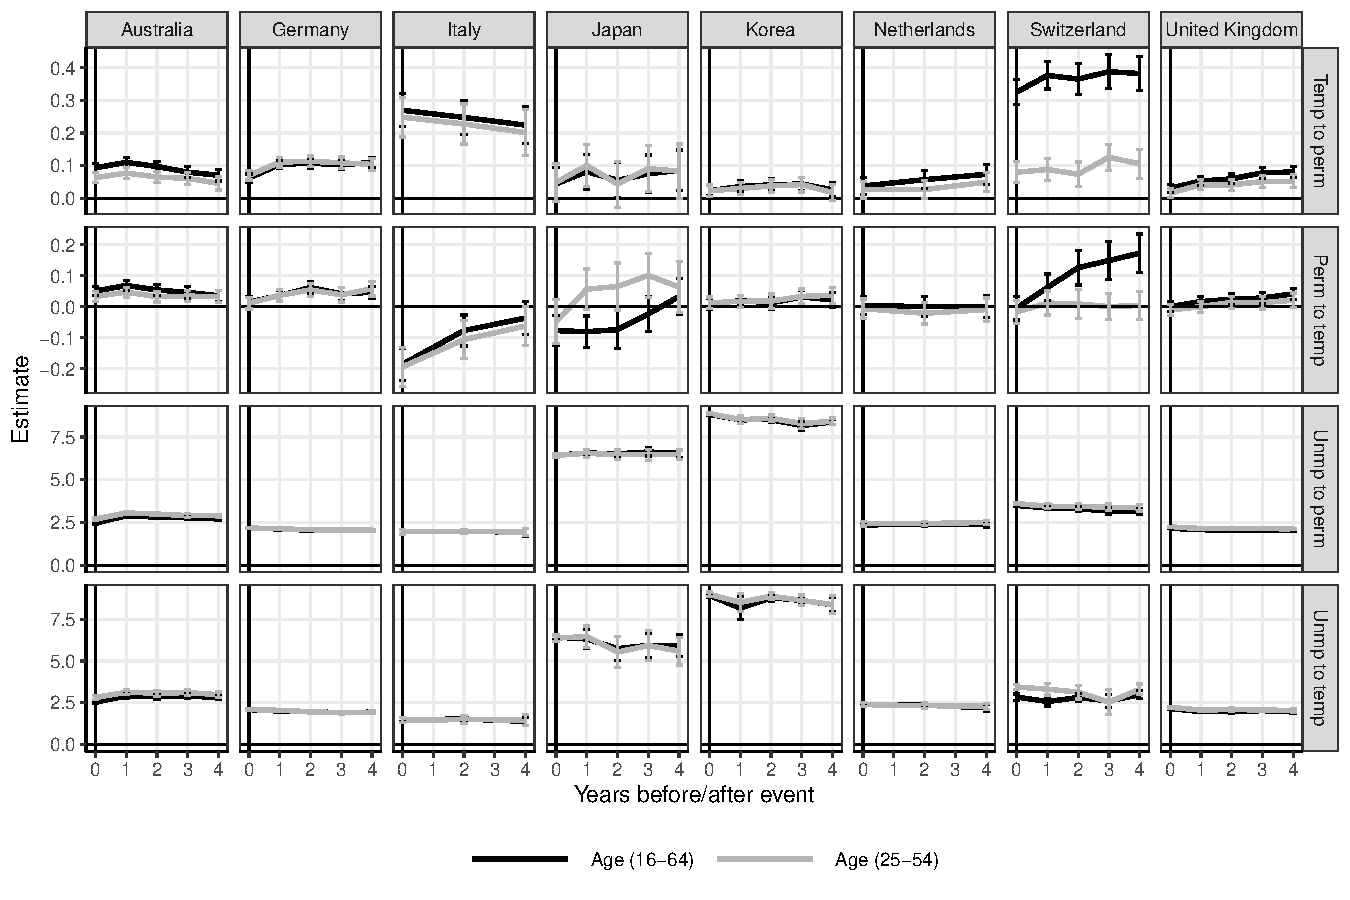
\includegraphics{../../../graphs/age_16_64/graph_sensitivity_age_post.pdf}}
    \label{graph_post_age_16_64}
\end{sidewaysfigure}

\begin{sidewaysfigure}[h!]
    \caption{Switzerland -- Differences in reason for temporary employment by sample age group}
    \resizebox{\textwidth}{!}{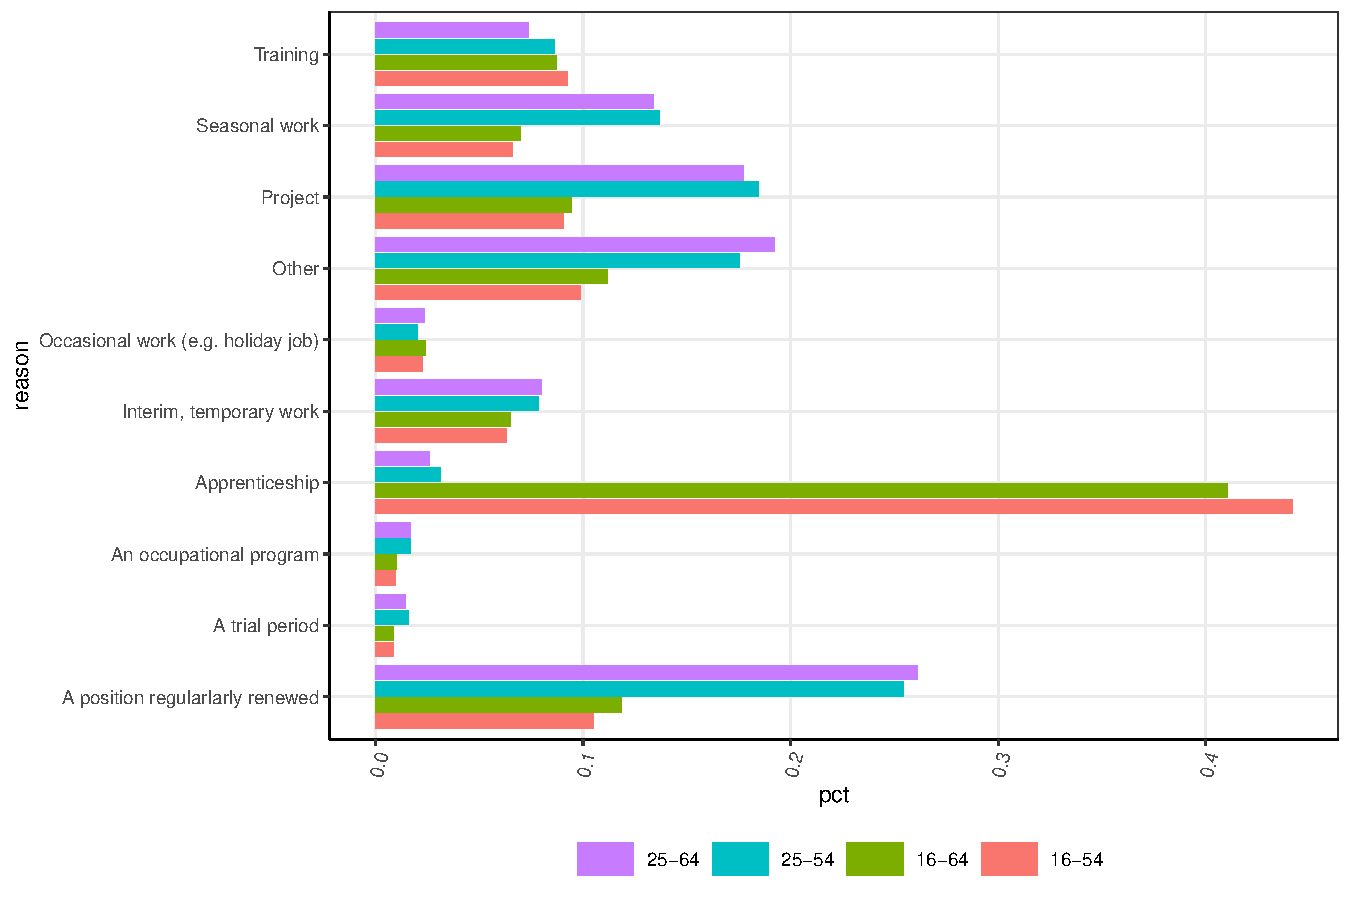
\includegraphics{../../../graphs/age_16_64/graph_ch_compare_sample_age.pdf}}
    \label{graph_ch_compare_sample_age}
\end{sidewaysfigure}

\begin{sidewaysfigure}[!h]
    \caption{Compare sample with at least 3 (as in the paper) vs. 2 observations (compare to figure \ref{graph_contyp})}
    \resizebox{\textwidth}{!}{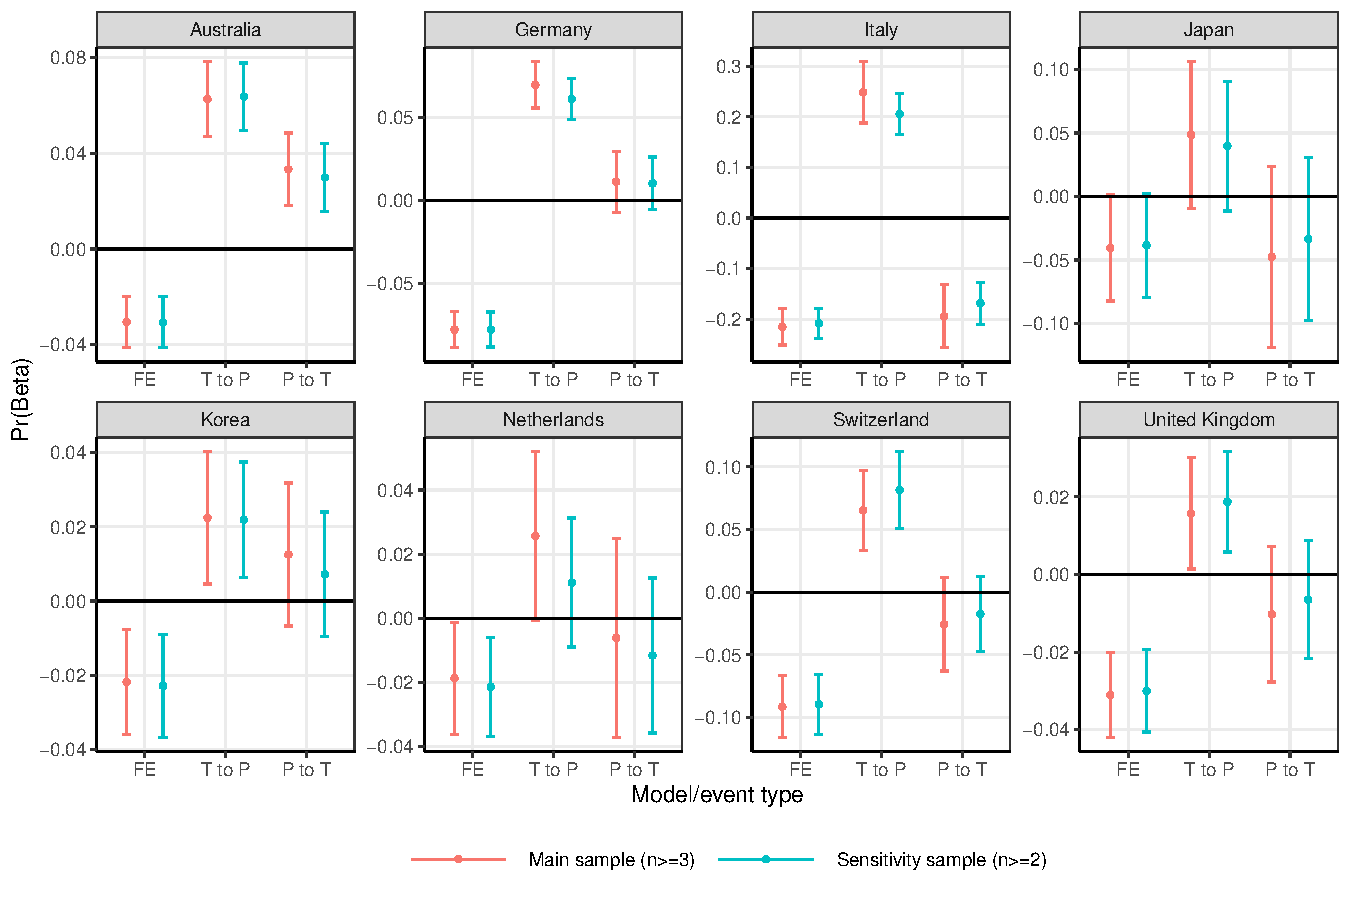
\includegraphics{../../../graphs/sample_2_years/graph_sensitivity_compare_contyp_sample_2_years.pdf}}
    \label{graph_sensitivity_compare_contyp_sample_2_years}
\end{sidewaysfigure}

\begin{sidewaysfigure}[!h]
    \caption{Compare sample with at least 3 (as in the paper) vs. 2 observations (compare to figure \ref{graph_unmp})}
    \resizebox{\textwidth}{!}{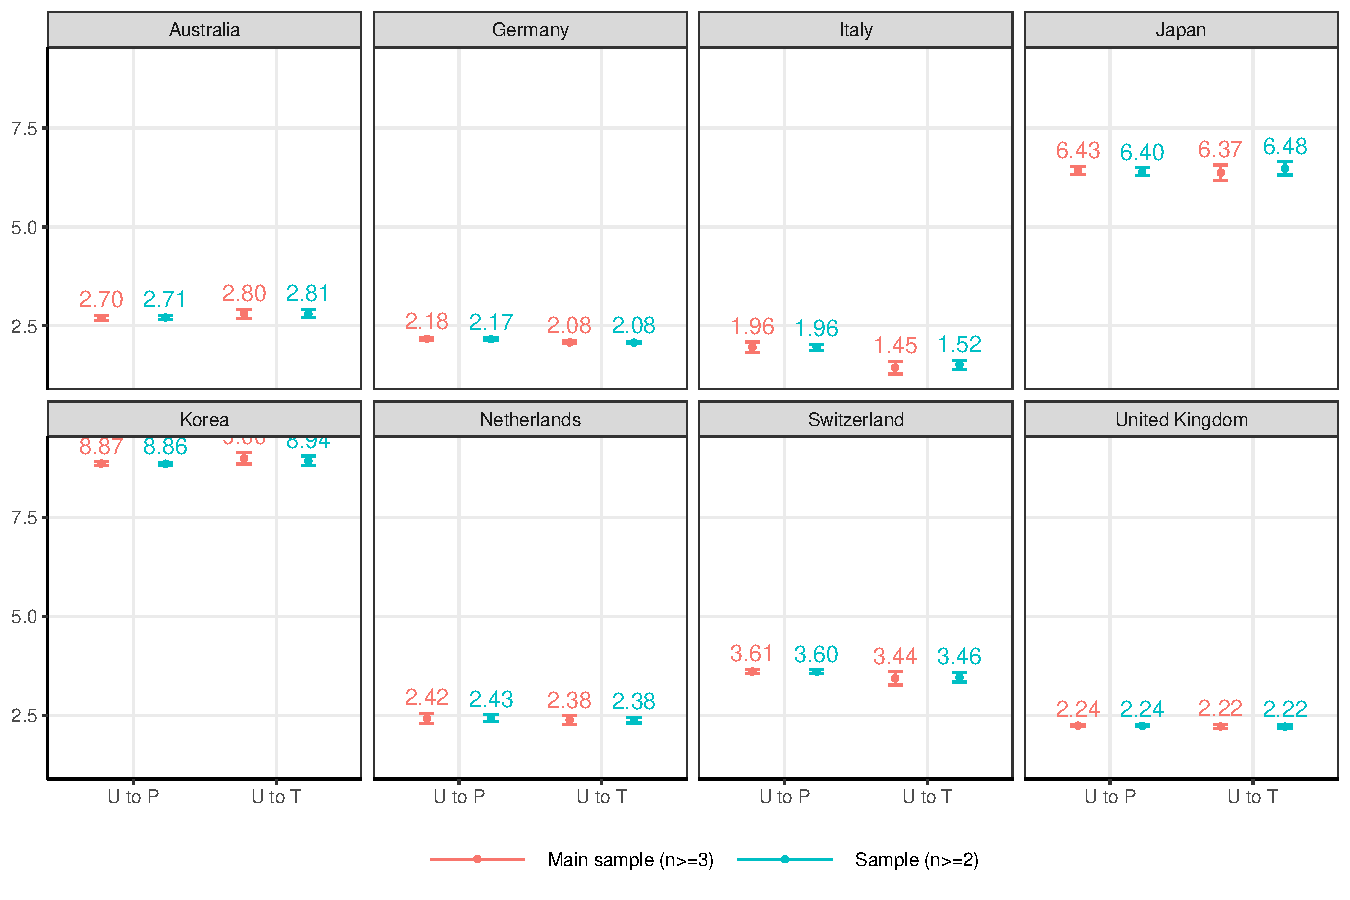
\includegraphics{../../../graphs/sample_2_years/graph_sensitivity_compare_unmp_sample_2_years.pdf}}
    \label{graph_sensitivity_compare_unmp_sample_2_years}
\end{sidewaysfigure}

\begin{sidewaysfigure}[!h]
    \caption{Graphical effect of transition on wages over time with different hours samples (as compared to figures \ref{graph_contyp_post} and  \ref{graph_unmp_post})}
    \resizebox{\textwidth}{!}{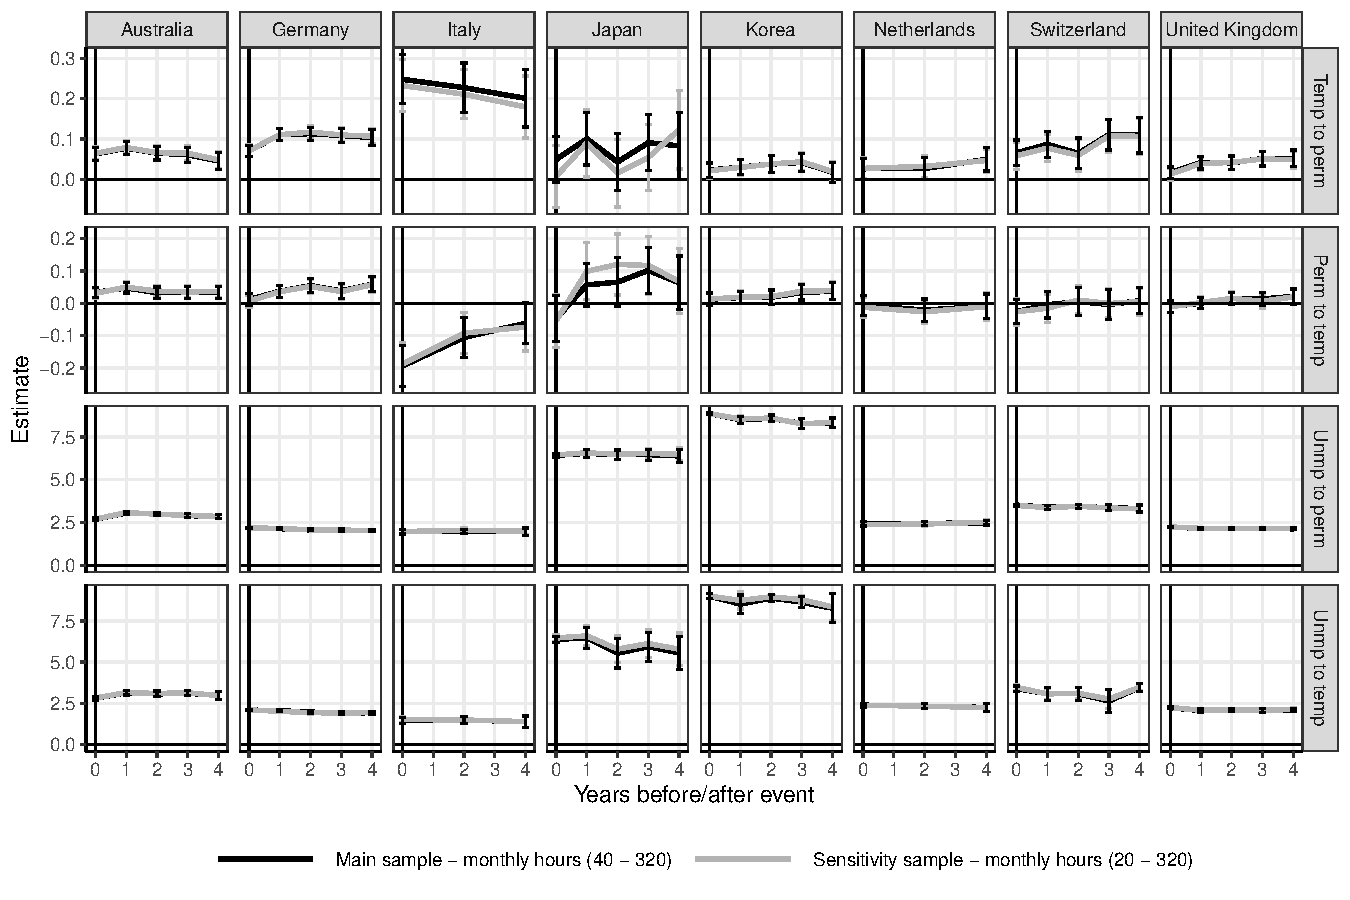
\includegraphics{../../../graphs/hours/graph_sensitivity_hours_post.pdf}}
    \label{graph_post_hours}
\end{sidewaysfigure}

\begin{sidewaysfigure}[!h]
    \caption{Graphical effect of transitions out of unemployment on wages over time with different samples (as compared to figure \ref{graph_unmp_post})}
    \resizebox{\textwidth}{!}{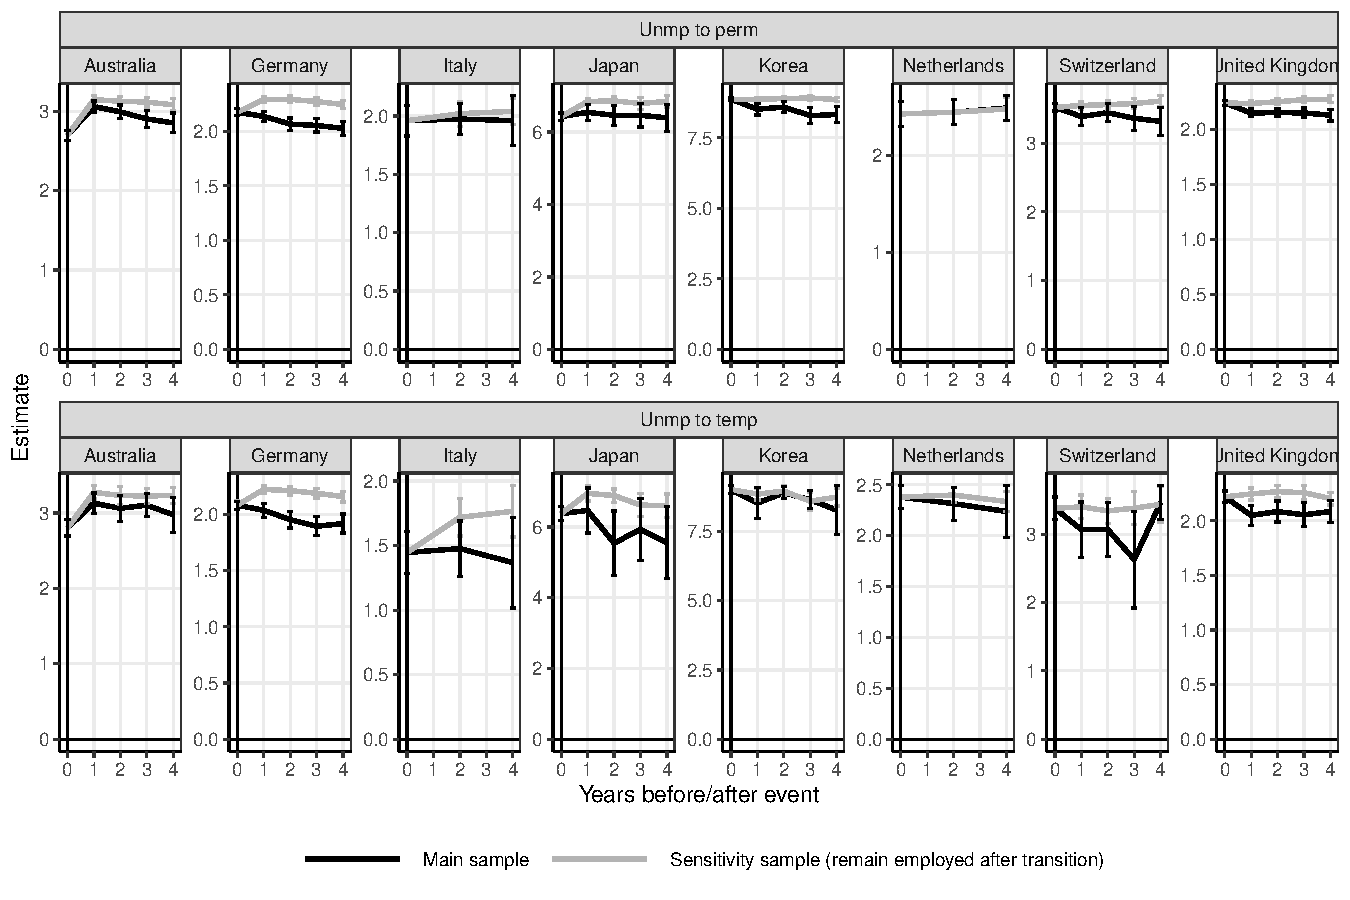
\includegraphics{../../../graphs/employed/graph_sensitivity_employed_post_2.pdf}}
    \label{graph_post_employed_2}
\end{sidewaysfigure}

\begin{sidewaysfigure}[!h]
    \caption{Graphical effect of transitions out of unemployment on wages over time with different samples (as compared to figure \ref{graph_unmp_post})}
    \resizebox{\textwidth}{!}{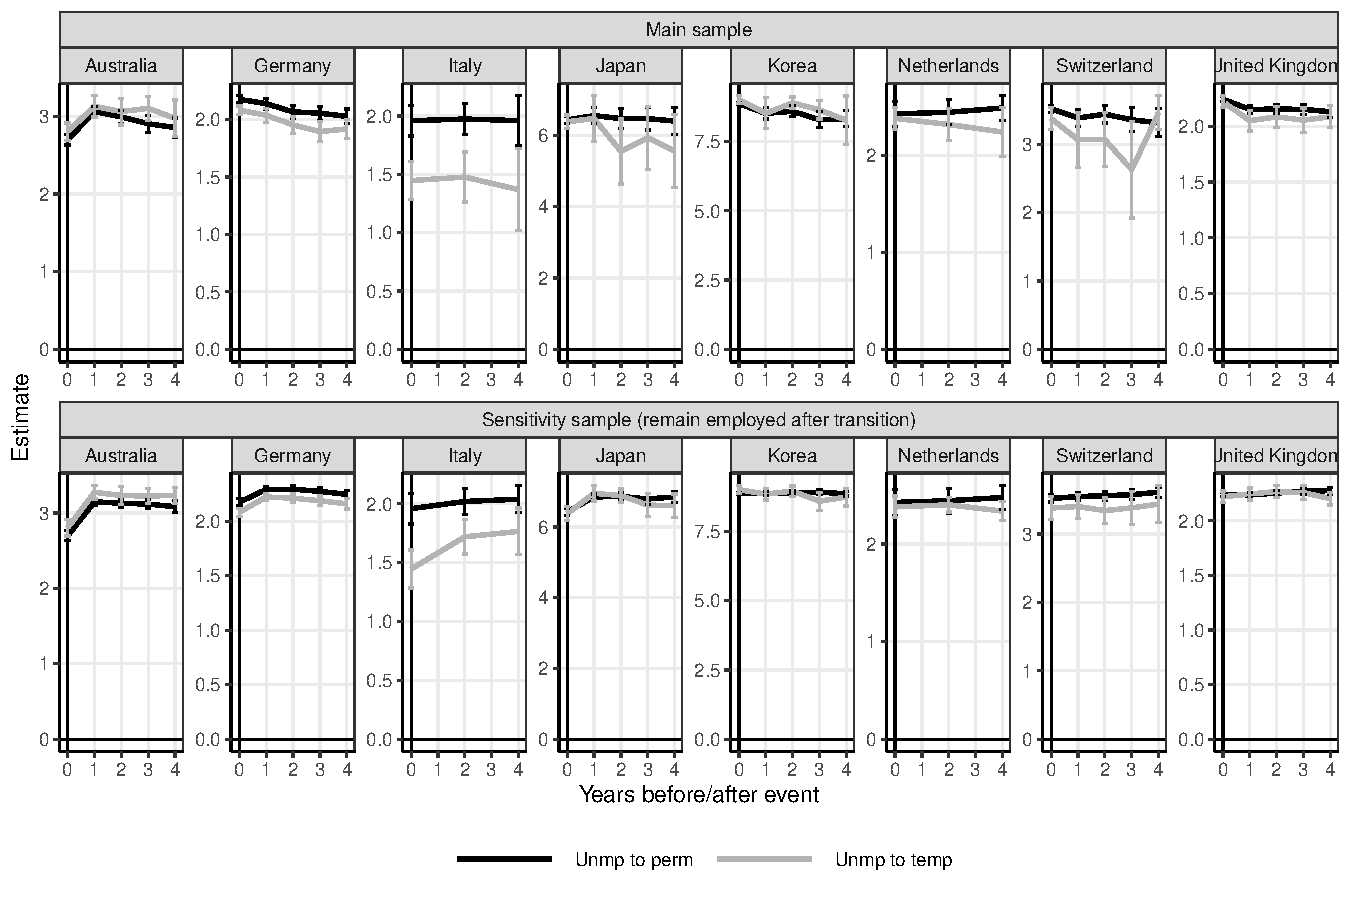
\includegraphics{../../../graphs/employed/graph_sensitivity_employed_post_1.pdf}}
    \label{graph_post_employed_1}
\end{sidewaysfigure}



%%%%%%%%%%%%%%%%%%%%%%%%%%%%%%%%%%%%%%%%%%
%%%%%%%%%%%%%%%%%%%%%%%%%%%%%%%%%%%%%%%%%%
%%%%%%%%%%%%%%%%%%%%%%%%%%%%%%%%%%%%%%%%%%
%%%%%%%%%%%%%%%%%%%%%%%%%%%%%%%%%%%%%%%%%%
\clearpage
\section{Appendix: Sensitivity to model specification}\label{appendix:sensitivity_model}
\setcounter{table}{0}
\setcounter{figure}{0}
\renewcommand*\thetable{\Alph{section}.\arabic{table}}
\renewcommand*\thefigure{\Alph{section}.\arabic{figure}}
\renewcommand{\theHfigure}{\Alph{section}.\arabic{table}}
\renewcommand{\theHtable}{\Alph{section}.\arabic{figure}}

In this section, we test the sensitivity of our model specification.  

First, we estimate both models \ref{eq:model_afe_temp} and \ref{eq:model_afe_unmp}.  We refer to these models as asymmetric fixed effect with dummy impact functions (AFE + DIF).  According to Rüttenauer and Ludwig \citeyearpar{ruttenauer_fixed_2020} the FE estimation may overestimate the treatment effect as it does not model confounding by heterogeneous trends, whereas FEIS may underestimate the treatment effect as it may not properly distinguish the treatment effect from heterogeneous trends. For these reasons, we ran sensitivity check by estimating models \ref{eq:model_afe_temp} and \ref{eq:model_afe_unmp} with FEIS + DIF.  These are shown in figures \ref{graph_compare_model_feis}.  Results are qualitatively similar.

Second, we compare results using a sample with multiple events (as in the main paper) to a sample with only the first event.  These are shown in figures \ref{graph_sensitivity_single_multiple_events}.  Results are qualitatively similar.

Third, we compare results in the main sample specification to a sensitivity sample where we drop or censor pre-treatment observations before the reference period and post-treatment variables greater than 4 periods after the event.  In annual data, pre-treatment observations are less than 1 period before the event and 2 periods before the event in biannual data.  Therefore, in the sensitivity sample, 0 refers only to for all observations that did not experience a given event.  In the main sample, 0 refers both to individuals who either did not experience a given event or experienced the event at least 3 periods before.  This is shown in figure \ref{graph_sensitivity_post_censoring}.  Results are qualitatively similar.

\begin{sidewaysfigure}
    \caption{Methods: FE + DIF (as in the paper) vs. FEIS + DIF}
    \resizebox{\textwidth}{!}{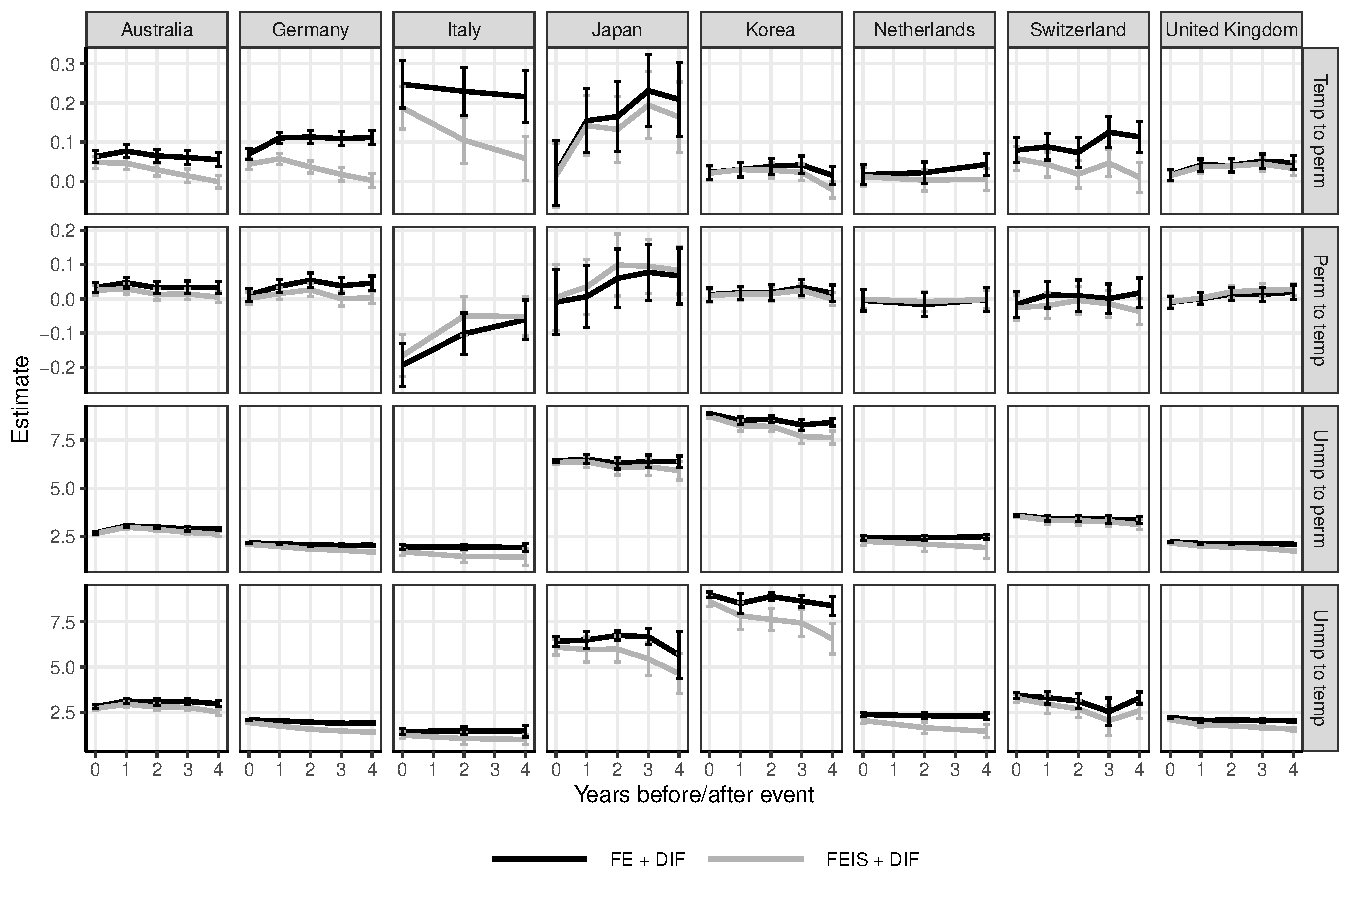
\includegraphics{../../../graphs/sensitivity/graph_compare_model_feis_paper.pdf}}
    \label{graph_compare_model_feis}
\end{sidewaysfigure}

\begin{sidewaysfigure}[!h]
    \caption{Compare multiple events (as in the paper) vs. first, single event}
    \resizebox{\textwidth}{!}{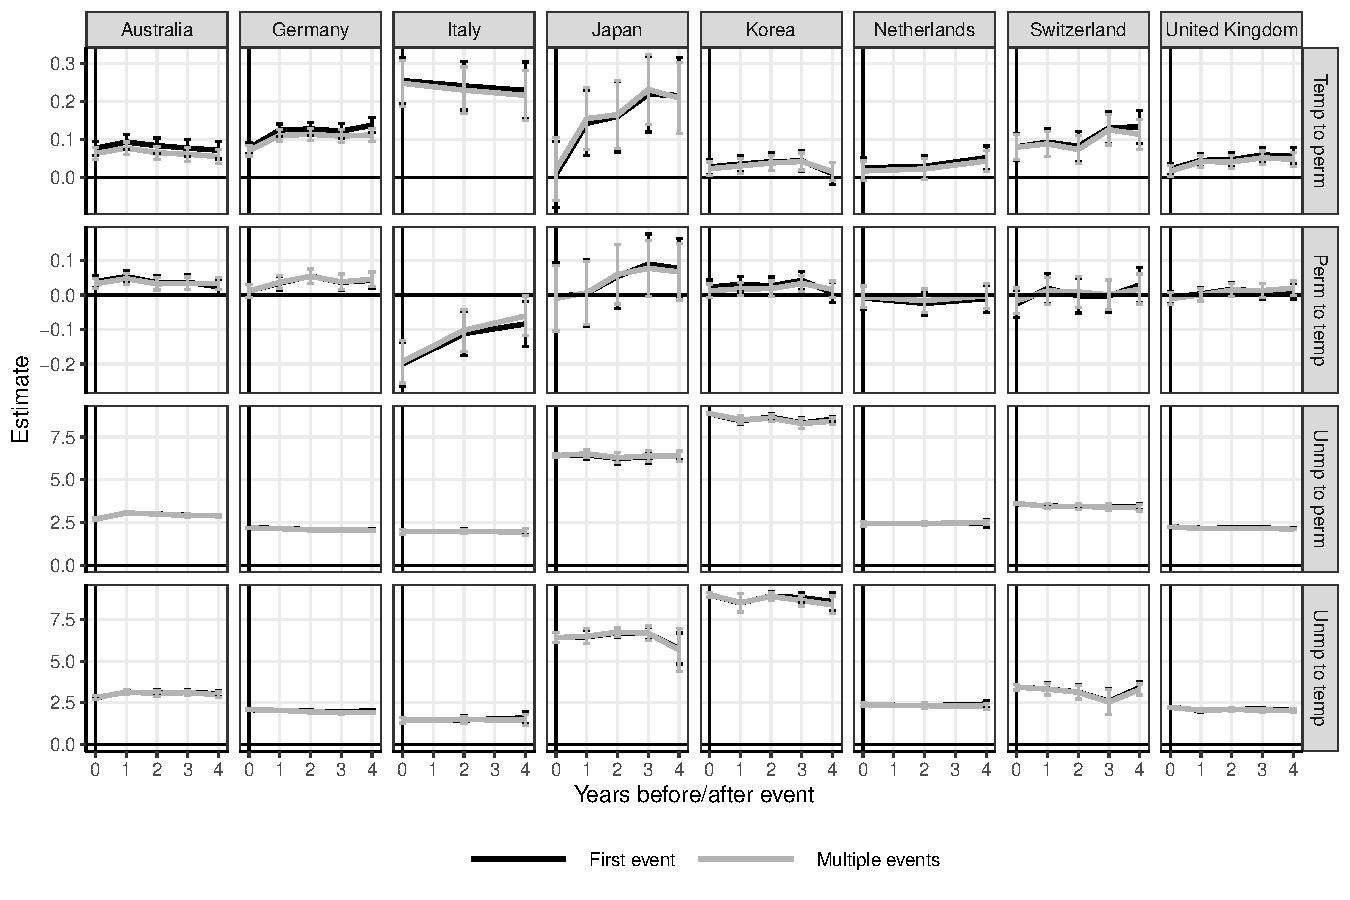
\includegraphics{../../../graphs/sensitivity/graph_sensitivity_single_multiple_events_paper.pdf}}
    \label{graph_sensitivity_single_multiple_events}
\end{sidewaysfigure}{}

% \begin{sidewaysfigure}[h!]
%     \caption{Effect of transitions between contract type on wages at point in time (as compared to figure \ref{graph_contyp})}
%     \resizebox{\textwidth}{!}{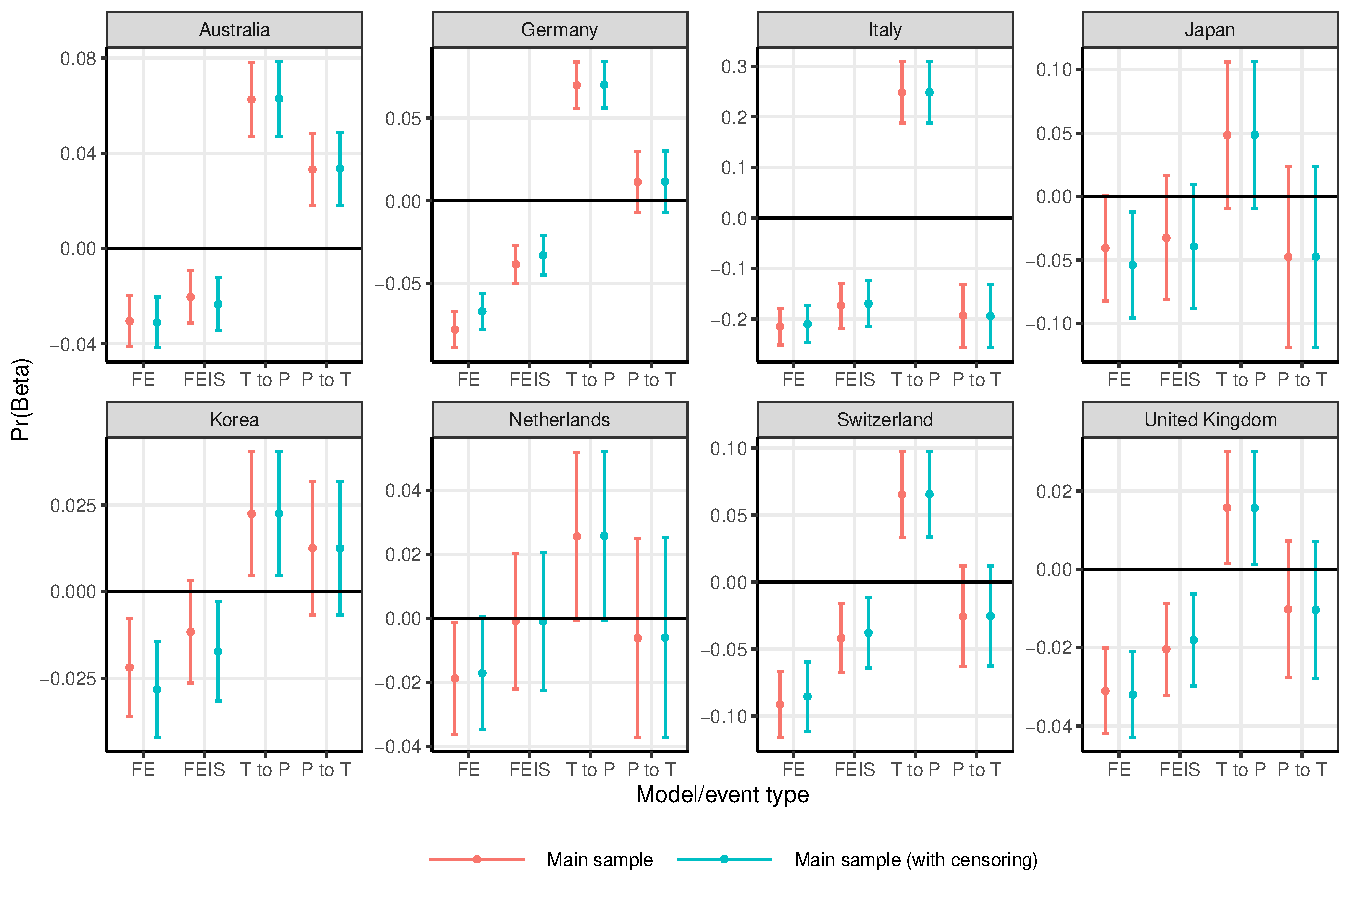
\includegraphics{../../../graphs/censoring/graph_sensitivity_compare_contyp_censoring.pdf}}
%     \label{graph_sensitivity_contyp_censoring}
% \end{sidewaysfigure}

% \begin{sidewaysfigure}
%     \caption{Effect of transitions out of unemployment by contract type on wages at point in time (as compared to figure \ref{graph_unmp})}
%     \resizebox{\textwidth}{!}{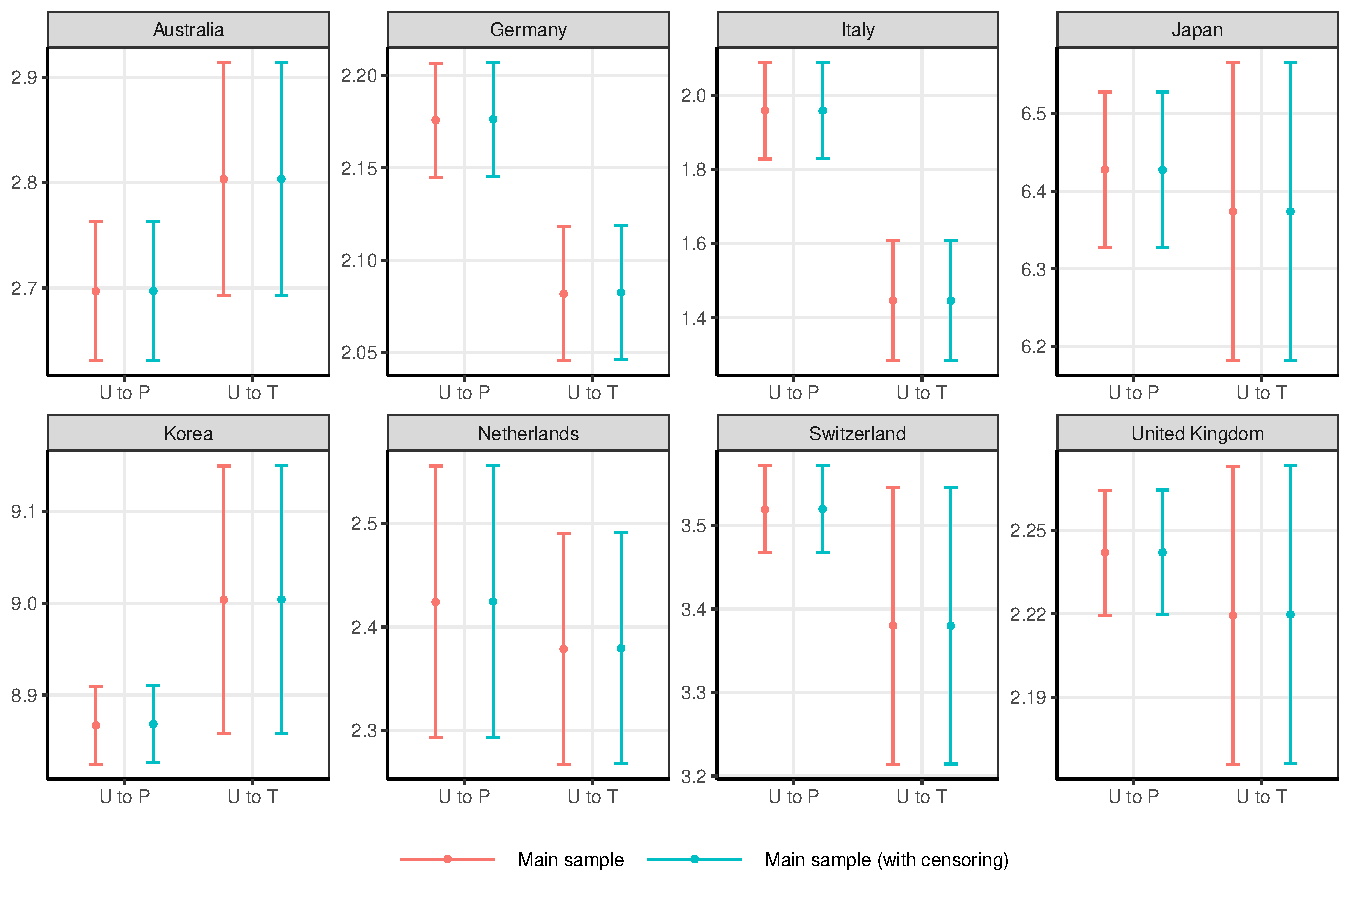
\includegraphics{../../../graphs/censoring/graph_sensitivity_compare_unmp_censoring.pdf}}
%     \label{graph_sensitivity_unmp_censoring}
% \end{sidewaysfigure}

\begin{sidewaysfigure}
    \caption{Graphical effect of transition on wages over time (as compared to figures \ref{graph_contyp_post} and  \ref{graph_unmp_post})}
    \resizebox{\textwidth}{!}{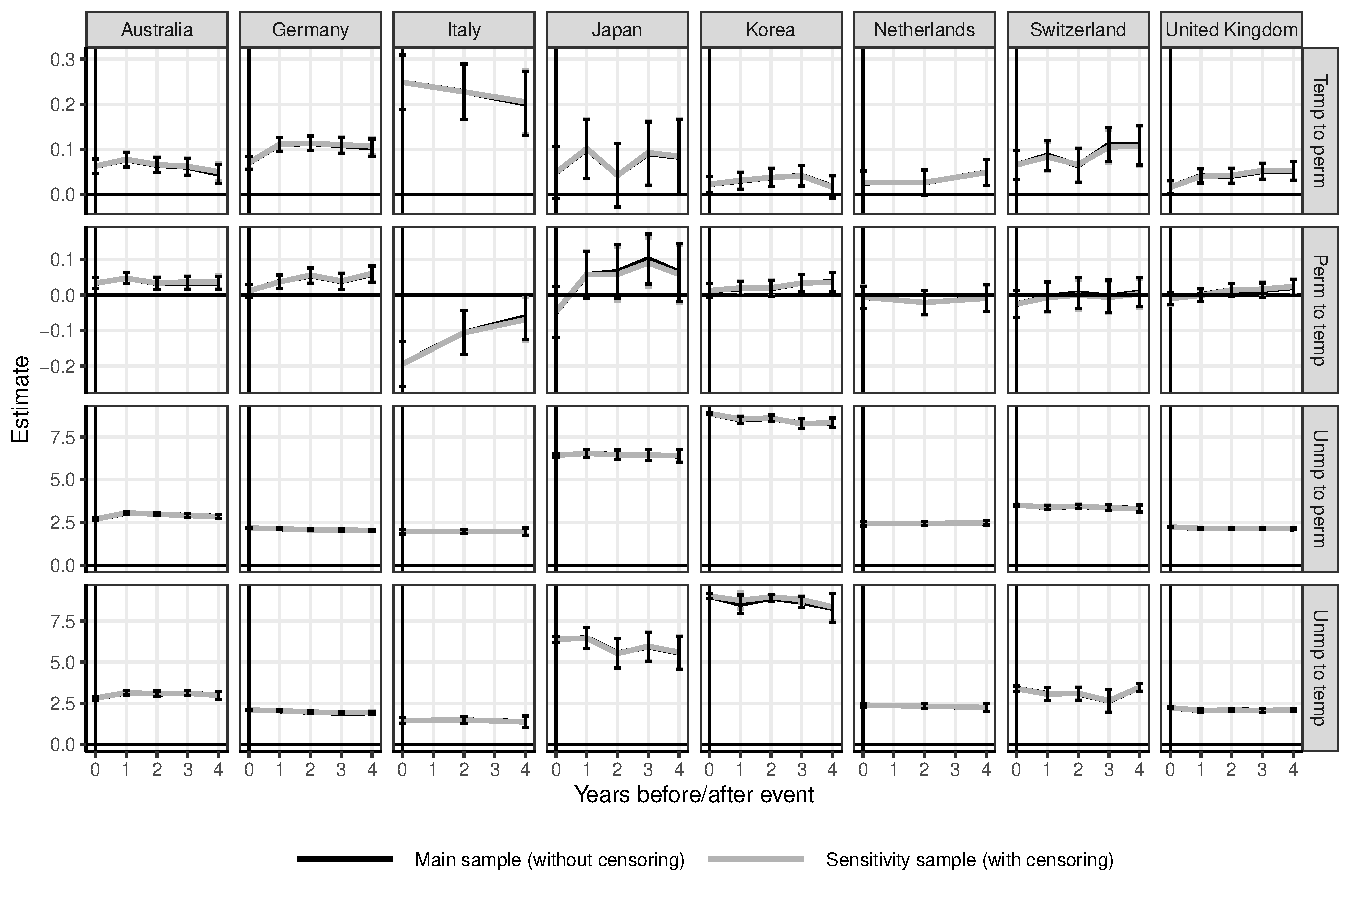
\includegraphics{../../../graphs/censoring/graph_sensitivity_censoring_post.pdf}}
    \label{graph_sensitivity_post_censoring}
\end{sidewaysfigure}


%%%%%%%%%%%%%%%%%%%%%%%%%%%%%%%%%%%%%%%%%%
%%%%%%%%%%%%%%%%%%%%%%%%%%%%%%%%%%%%%%%%%%
%%%%%%%%%%%%%%%%%%%%%%%%%%%%%%%%%%%%%%%%%%
%%%%%%%%%%%%%%%%%%%%%%%%%%%%%%%%%%%%%%%%%%
\clearpage
\section{Appendix: Results sensitivity}\label{appendix:sensitivity_variable}
\setcounter{table}{0}
\setcounter{figure}{0}
\renewcommand*\thetable{\Alph{section}.\arabic{table}}
\renewcommand*\thefigure{\Alph{section}.\arabic{figure}}
\renewcommand{\theHfigure}{\Alph{section}.\arabic{table}}
\renewcommand{\theHtable}{\Alph{section}.\arabic{figure}}

In this appendix, we examine the robustness of the results to distinct model specifications or definitions of event.  In Australia and in the United Kingdom, we compare different definitions of temporary employment (Figure \ref{graph_sensitivity_AU} and \ref{graph_sensitivity_AU}, respectively).  Further, in the Netherlands, we also compare results from the LSP to the LISS (Figure \ref{graph_sensitivity_NE}).  



\begin{sidewaysfigure}[!h]
    \caption{Australia: All temporary (incl. casual) vs. FTC only (as in the paper)}
    \resizebox{\textwidth}{!}{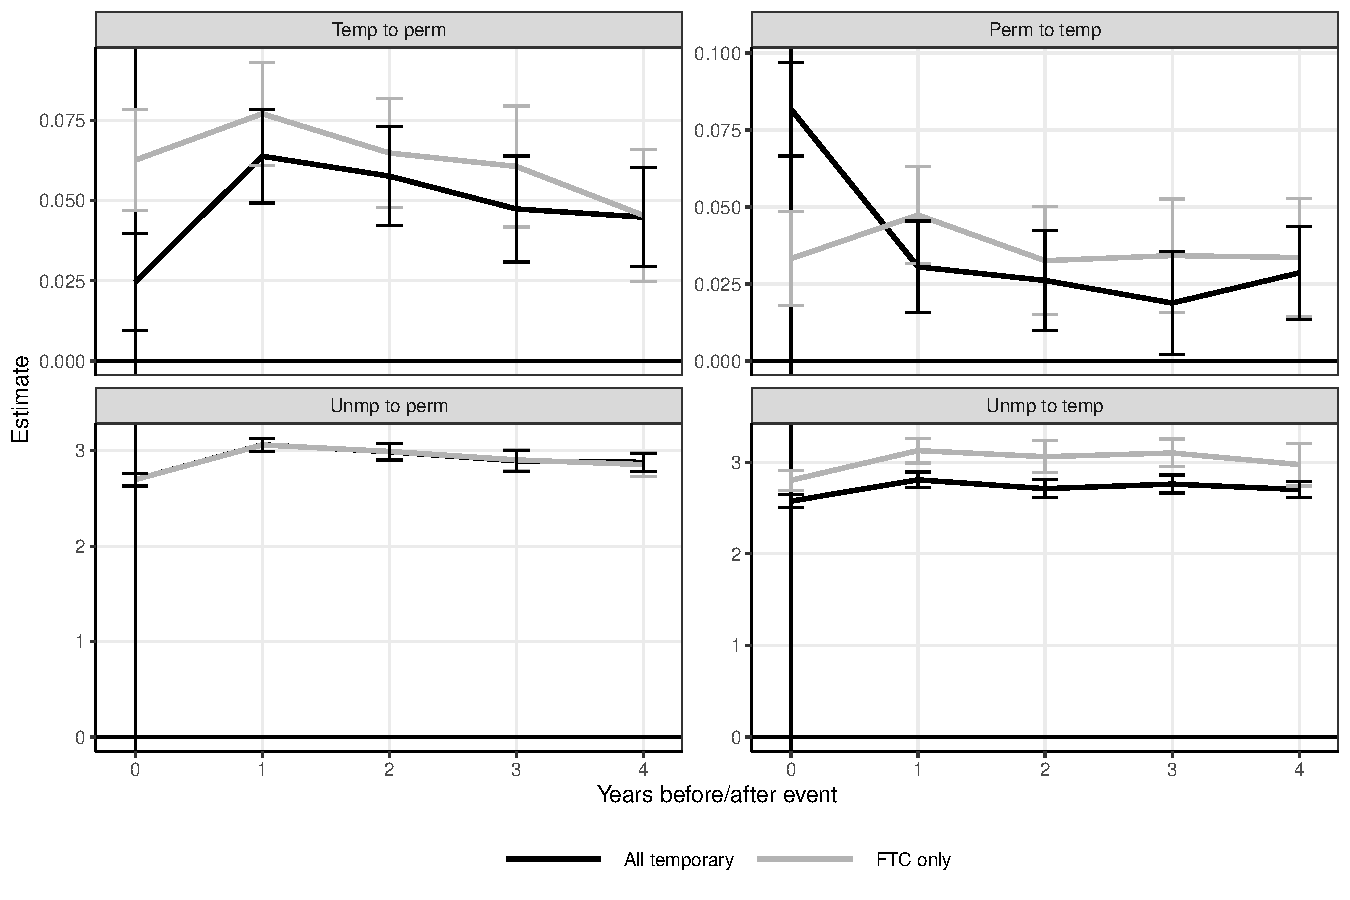
\includegraphics{../../../graphs/sensitivity/graph_sensitivity_AU_paper.pdf}}
    \label{graph_sensitivity_AU}
\end{sidewaysfigure}


\begin{sidewaysfigure}
    \caption{United Kingdom: All temporary (as in the paper) vs. FTC only}
    \resizebox{\textwidth}{!}{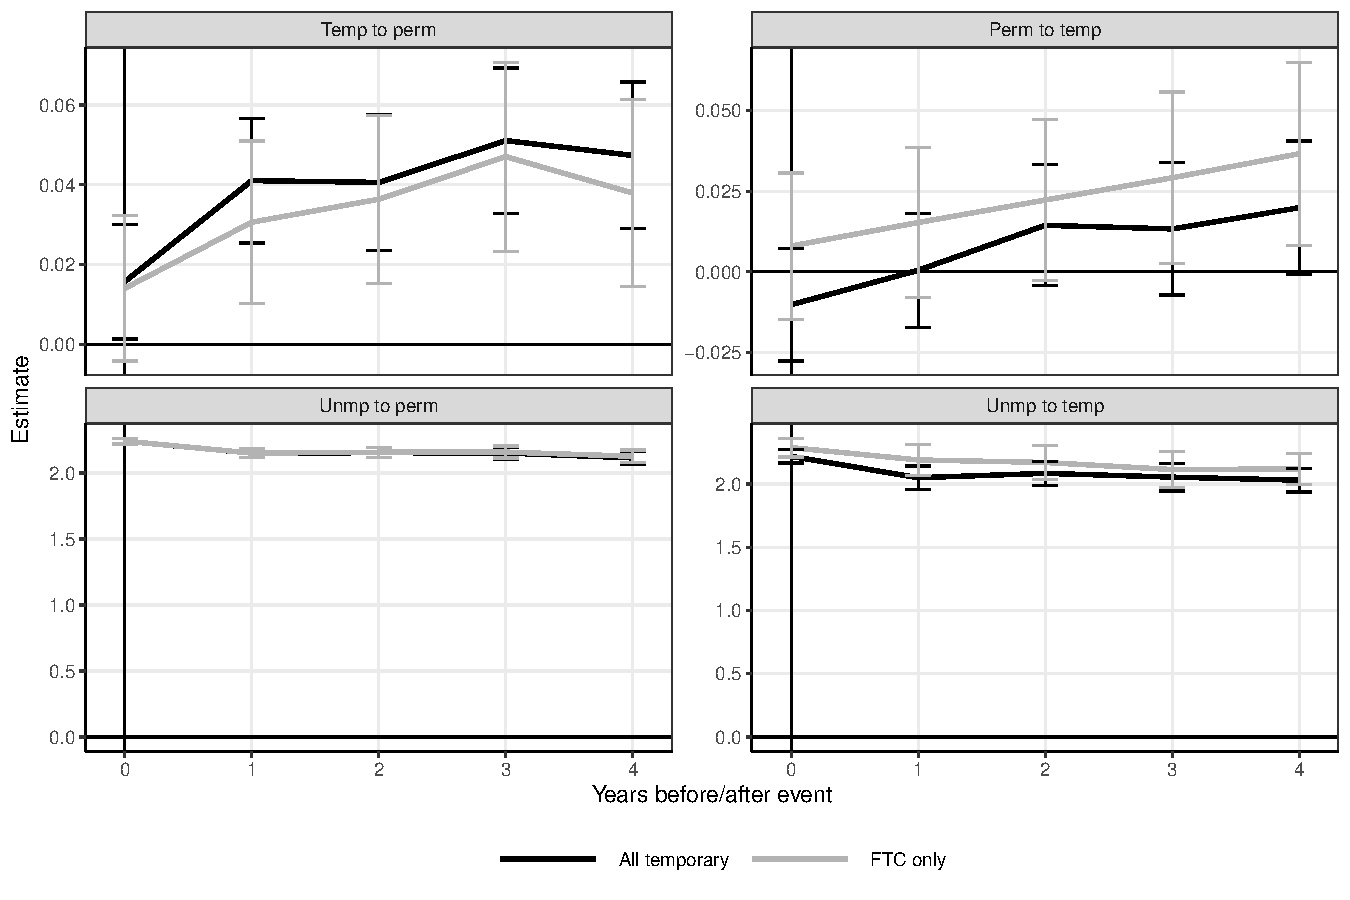
\includegraphics{../../../graphs/sensitivity/graph_sensitivity_UK_paper.pdf}}
    \label{graph_sensitivity_UK}
\end{sidewaysfigure}

\begin{sidewaysfigure}
    \caption{Netherlands: LSP (as in the paper) vs. LISS}
    \resizebox{\textwidth}{!}{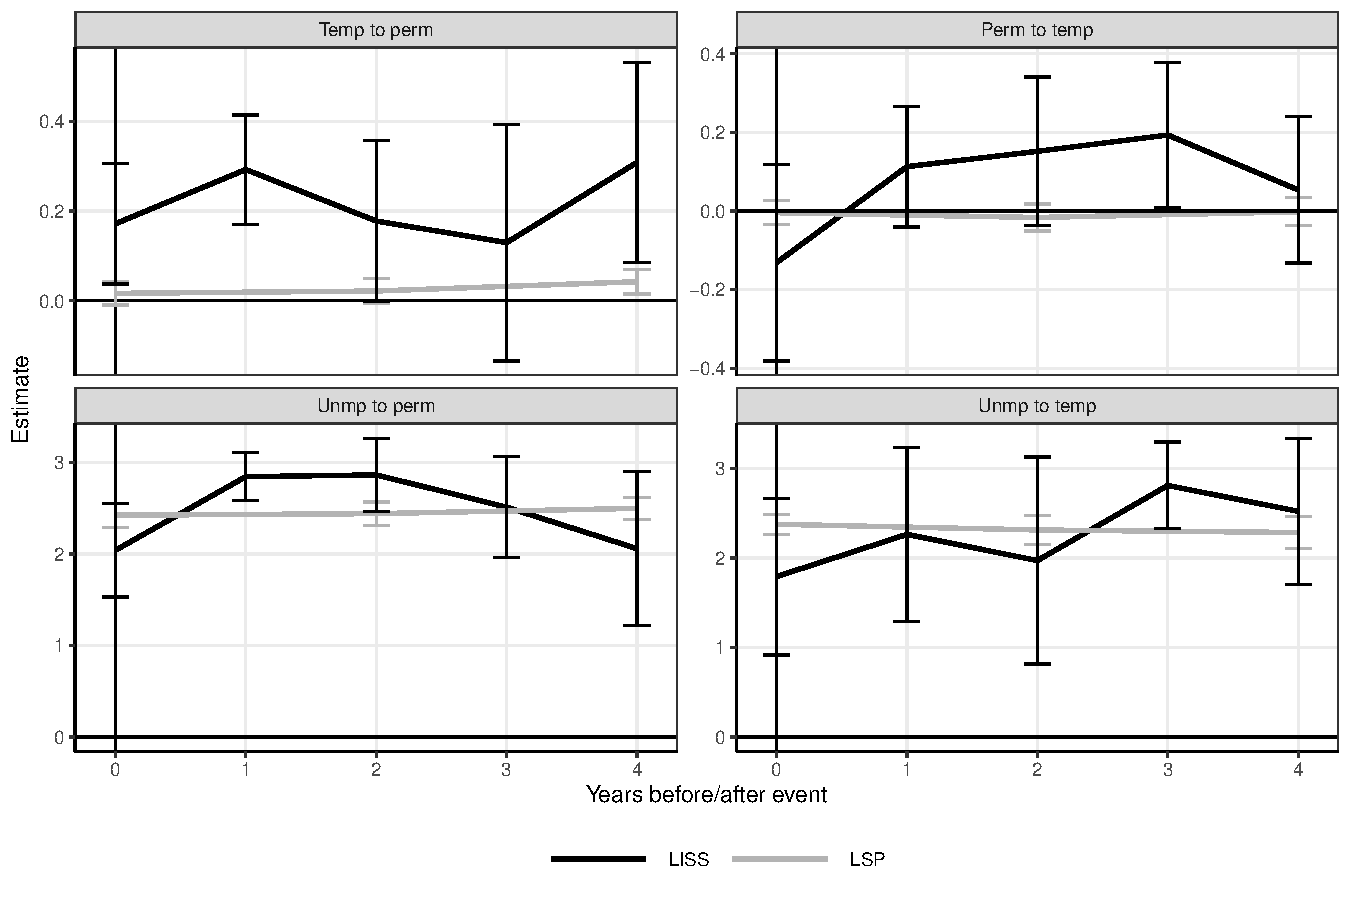
\includegraphics{../../../graphs/sensitivity/graph_sensitivity_NE_paper.pdf}}
    \label{graph_sensitivity_NE}
\end{sidewaysfigure}



%%%%%%%%%%%%%%%%%%%%%%%%%%%%%%%%%%%%%%%%%%
%%%%%%%%%%%%%%%%%%%%%%%%%%%%%%%%%%%%%%%%%%
%%%%%%%%%%%%%%%%%%%%%%%%%%%%%%%%%%%%%%%%%%
%%%%%%%%%%%%%%%%%%%%%%%%%%%%%%%%%%%%%%%%%%
\clearpage
\setcounter{table}{0}
\setcounter{figure}{0}
\renewcommand*\thetable{\Alph{section}.\arabic{table}}
\renewcommand*\thefigure{\Alph{section}.\arabic{figure}}
\renewcommand{\theHfigure}{\Alph{section}.\arabic{table}}
\renewcommand{\theHtable}{\Alph{section}.\arabic{figure}}

\section{Appendix: Results heterogeneity}\label{appendix:sensitivity_heterogeneity}

We conducted a series of robustness checks, which we broadly split into two categories.  In appendix \ref{appendix:sensitivity_variable}, we examine the robustness of the results to distinct model specifications or definitions of event.  In this appendix, we examine the robustness of the results to distinct heterogeneous groups, as shown in Appendix \ref{appendix:sensitivity_heterogeneity}.  Figure \ref{graph_post_event_age_cat} compares age groups (25-34, 35-44, and 45-54), figure \ref{graph_post_event_edu_cat} compares education groups (less than secondary, secondary, and more than secondary education), and figure \ref{graph_post_event_gender} compares results for men and women.  All results are qualitatively similar.

\begin{sidewaysfigure}[!h]
    \caption{Figures \ref{graph_contyp_post} and \ref{graph_unmp_post}, by age category}
    \resizebox{\textwidth}{!}{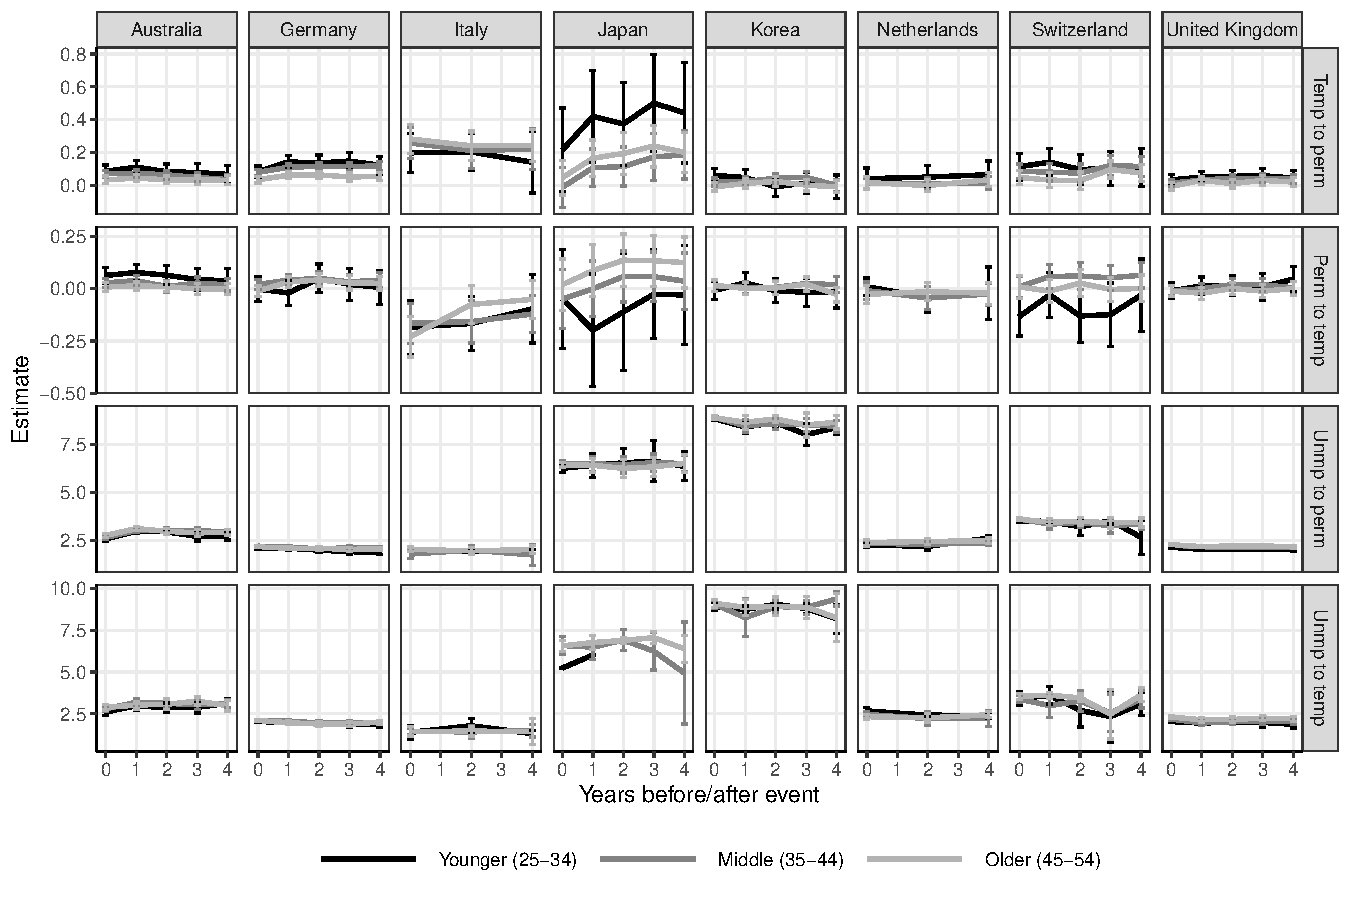
\includegraphics{../../../graphs/heterogeneity/graph_post_event_age_cat.pdf}}
    \label{graph_post_event_age_cat}
\end{sidewaysfigure}

\begin{sidewaysfigure}[!h]
    \caption{Figures \ref{graph_contyp_post} and \ref{graph_unmp_post}, by education category}
    \resizebox{\textwidth}{!}{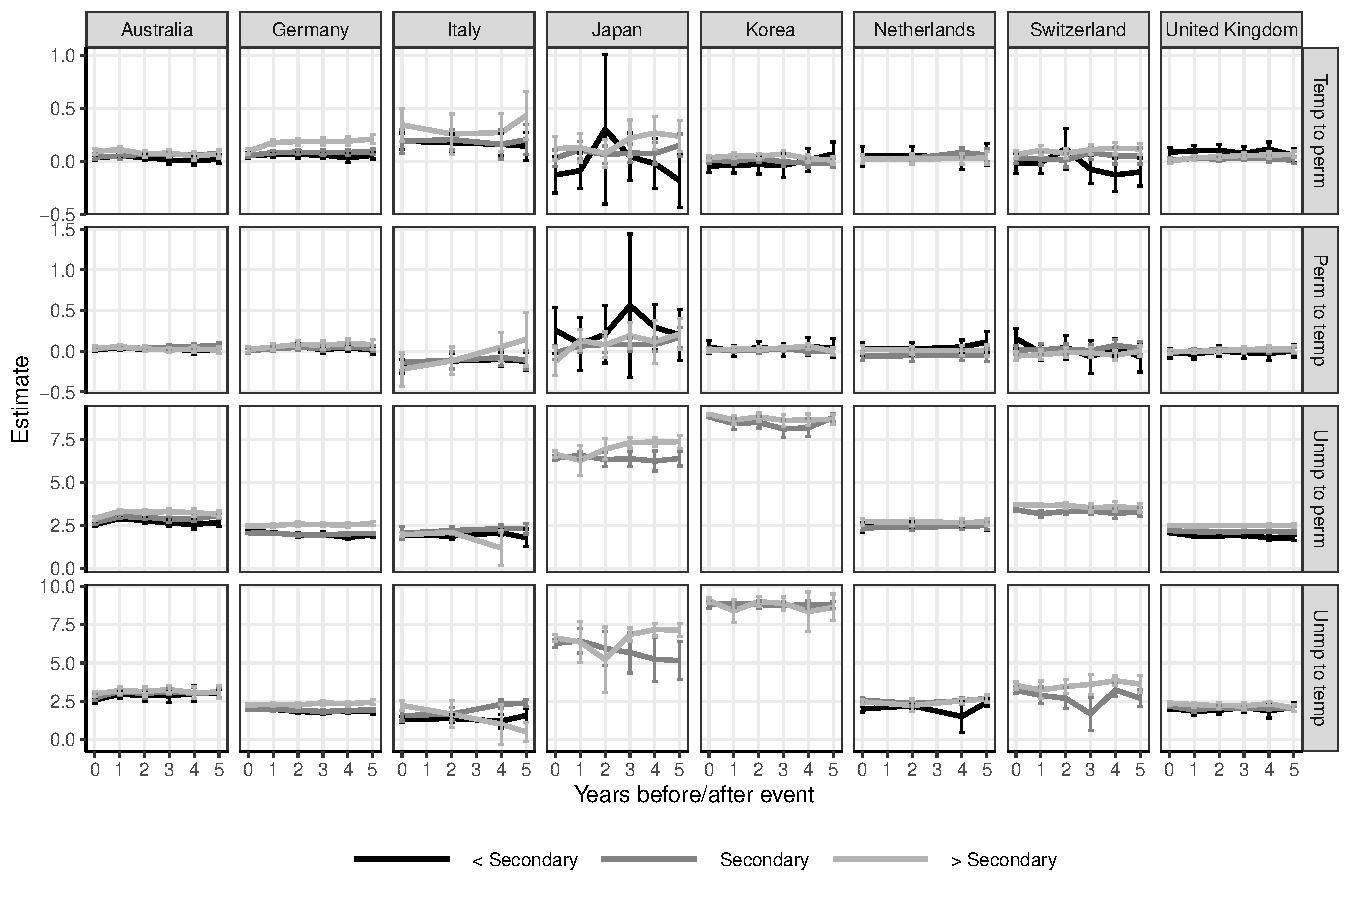
\includegraphics{../../../graphs/heterogeneity/graph_post_event_edu_cat.pdf}}
    \label{graph_post_event_edu_cat}
\end{sidewaysfigure}

\begin{sidewaysfigure}[!h]
    \caption{Figures \ref{graph_contyp_post} and \ref{graph_unmp_post}, by gender}
    \resizebox{\textwidth}{!}{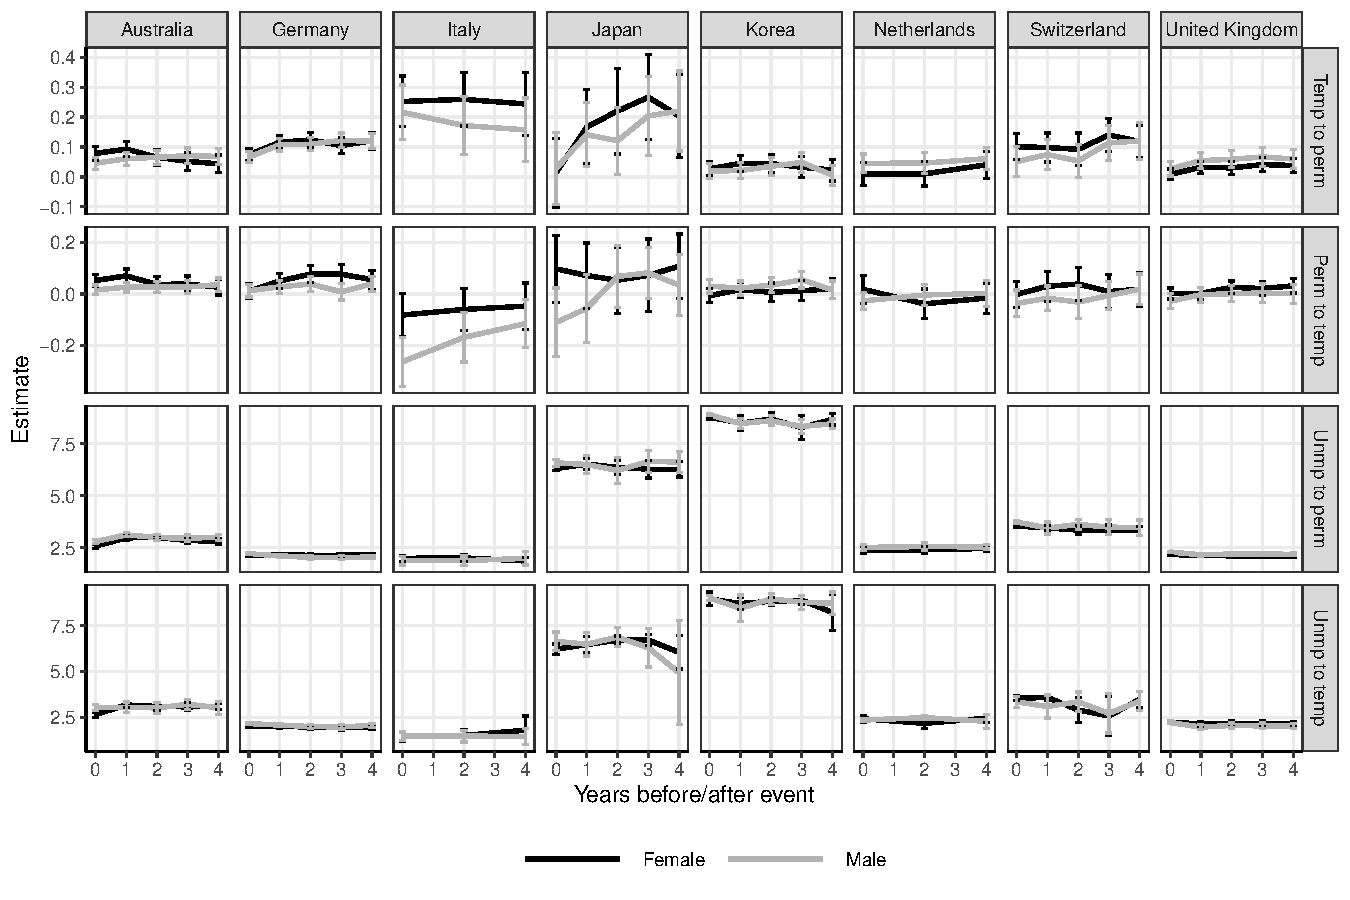
\includegraphics{../../../graphs/heterogeneity/graph_post_event_gender.pdf}}
    \label{graph_post_event_gender}
\end{sidewaysfigure}


